\documentclass[a5paper]{article}

\usepackage{fontspec}
\setmonofont[Scale=0.9]{DejaVuSansCondensed} % Not condensed enough
%\setmonofont{HelveticaLTStd-LightCond}
%\setmonofont{FagoOfficeSerif-Regular}  % Too dark
%\setmonofont{FuturaStd-Light}
%\setmonofont{Interstate Cond Mono - Lgt}

\usepackage{hyperref}
\usepackage{amsmath,amssymb,stmaryrd}
\usepackage{paralist}


\iftrue  % For screen
\usepackage[
  paperwidth=9cm,
  paperheight=16cm,
  width=8.5cm,
  height=15.5cm,
  left=.25cm,
  includefoot,
  foot=.75cm,
]{geometry}
\else  % For print
\usepackage[
  paperwidth=4.25in,
  paperheight=6.875in,
  width=3.25in,
  height=6.375in,
  left=.5in,
  top=.25in,
  includefoot,
  foot=.75cm,
]{geometry}
\fi

\usepackage{tikz}

\def\CC{\mathbf{C}}
\def\RR{\mathbf{R}}
\def\n#1{\left\|#1\right\|}
\let\epsilon\varepsilon
\DeclareMathOperator{\cov}{Cov}
\DeclareMathOperator{\tr}{Tr}

\parindent 0pt
\parskip .5em

\let\d\textbf
\let\leq\leqslant
\let\geq\geqslant
\let\le\leqslant
\let\ge\geqslant

\newenvironment{reference}{%
  \medskip\goodbreak
  \parskip 0pt
  \raggedright
  \leftskip 1em
  %\rightskip 1em  % This would undo \raggedright
  \obeylines
}{\par\medskip\goodbreak}

\providecommand{\tightlist}{%
  \setlength{\itemsep}{0pt}\setlength{\parskip}{0pt}}
\usepackage{enumitem}
\setlist{nosep,leftmargin=*}

\def\section#1{\clearpage{\vspace*{0cm}\LARGE\centering\bfseries #1\par\bigskip\bigskip}}
\def\subsection#1{{\par\bigskip\goodbreak\large\bfseries #1\par}}

\title{2025 in Machine Learning}
\author{Vincent \textsc{Zoonekynd} and GPT-5.1}
\date{December 2025}

\begin{document}
\maketitle
\thispagestyle{empty}
\clearpage
\sloppy

\section{Prompts}\label{prompt}

\textsc{Human --}
\itshape
When I read research papers, I write a summary of them, all in a big,
unsorted \LaTeX{} file. Every year, I review that file, identify the topics
of the papers I have read, and sort the papers accordiong to those
topics. I then write a higher-level summary of those summaries, entitled
``This year in Machine Learning'', with one section per topic. Can you
help me do it this year? You will find below:

-- Last year's higher-level
summary (``This year in machine learning, 2024 edition''), as an example
of my writing style, inside \texttt{<example></example>} tags;

-- This year's detailed summaries (the big \LaTeX{} file, for 2025),
inside \texttt{<papers></papers>} tags

Can you do the following:

1. Identify the topics

2. Sort the
papers into those topics. You may discard some of the papers, if they
are not interesting, or if my summary is not clear. Keep at least half
the papers. Keep the title of the papers, the authors, the year (only if
available -- do not invent it), and a summary; reformulate (simplify)
the summary

3. Write a summary for each of those topics, using the same
style as in the example. Do not invent the URLs.

4. If you have access
to web search, add the URLs of the papers if they are on arxiv or
openreview (link to the abstract; if they are not on arxiv/openreview,
do not provide a URL). Stop after each of those steps to let me review
the results and amend the instructions if I notice they were unclear.

Here is last year's high-level summary:\\
\texttt{<example></example>}

Here are the detailed summaries from this year:\\
\texttt{<papers></papers>}
\upshape

\begin{center}\rule{0.5\linewidth}{0.5pt}\end{center}

\textsc{Human --}
\itshape
\texttt{@output.tex} This file was converted from a markdown file, \texttt{@output.md},
which used a mixture of \LaTeX{} and unicode for the equations.
The conversion not only kept the Unicode, but also mangled some of the \LaTeX{}.
Can you fix the \LaTeX{} file to use proper \LaTeX{} for all the math, without any unicode?
\upshape

\begin{center}\rule{0.5\linewidth}{0.5pt}\end{center}

\textsc{Human --}
\itshape
That is good: the unicode problems are fixed.
But there are still a few \LaTeX{} issues:

-- Math code (in particular subscripts) outside any math environment;

-- Completely mangled equations: pandoc seems to have replaced some substripts by \verb|\emph|.
(You can see the original code in \texttt{@tmp/output.md}: it should be more readable.)

Can you fix those remaining issues?
\upshape

\begin{center}\rule{0.5\linewidth}{0.5pt}\end{center}

\textsc{Human --}
\itshape
That looks better, but quite often the math is between brackets, e.g.,
\verb|(\alpha)|, instead of
\verb|\(\alpha\)| or
\verb|$\alpha$|.
Can you fix those?
\upshape

\section{Problems}

\begin{itemize}
\tightlist
\item ChatGPT did not reproduce my style: there were too many equations, and the sections did not have the same structure.
  Next year, ask him to analyze my style, and produce a prompt to reproduce it.
  Then check the prompt, try it on a subset of the data, and amend it.
\item The Markdown produced by ChatGPT was (mostly) correct, but \texttt{pandoc} completely mangled the math,
  and added a lot of spurious \verb|\\| (in lists, and before and after math mode).
  Next year, ask ChatGPT to produce Markdown suitable for conversion in \LaTeX{} with pandoc
  (no unicode for the math, \verb|$...$| and \verb|$$...$$| for math instead of \verb|\(...\)| and \verb|\[...\]|,
  use inline math for all mathematical quantities, even single letters)
  or, better, ask it to directly produce \LaTeX{}.
\end{itemize}
\clearpage

\textsc{ChatGPT --}
\itshape
I'll proceed topic by topic. For each:

\begin{itemize}
\tightlist
\item
  I'll list the \textbf{papers kept} (title, authors, year if you had
  it) with a \textbf{simplified summary} in your style.
\item
  Then I'll give a \textbf{concise section-level summary} like in your
  PDF (but here as plain text \LaTeX-ish content).
\end{itemize}

I won't add URLs yet (that's step 4).
\upshape

\section{1. Anytime-valid inference, e-values, and sequential change
detection}\label{anytime-valid-inference-e-values-and-sequential-change-detection}

\subsection{Papers}\label{papers}

\textbf{Game theoretic statistics and sequential anytime valid inference
(SAVI): a martingale theory of evidence}\\
(ICML 2025 tutorial)

This tutorial formalizes statistical testing as a betting game. Under
the null, your wealth process must be a (super)martingale: its
expectation never exceeds the initial stake, for any stopping time.
Nonnegative martingales (test martingales) and their running maxima
define e-values, anytime-valid p-processes, and sequential tests that
remain valid under arbitrary peeking and stopping rules. Kelly betting
appears as the log-optimal strategy: it maximizes the almost sure
exponential growth rate of wealth, which matches a KL divergence between
null and alternative.

Composite nulls are handled via ``reverse information projections'' and
numeraires: special e-variables that are log-optimal and characterize
the effective null by convex duality. The tutorial also shows how to
build confidence sequences (sequential confidence intervals with uniform
coverage in time) by turning families of betting strategies into
e-processes indexed by parameters, and then declaring as ``plausible''
those parameters for which wealth has not grown too much.

\begin{center}\rule{0.5\linewidth}{0.5pt}\end{center}

\textbf{E-detectors: a nonparametric framework for sequential change
detection}\\
J. Shin et al.~(2024)

E-detectors adapt e-process ideas to change-point detection. Under a
no-change null (all data from some $P\in\mathcal{P}$), an e-detector is a process $M_t$
whose expectation is at most the expected alarm time for any stopping
rule. They construct e-detectors from families of e-processes that
``re-start'' at each possible change point $j$ (e$_j$-processes), and combine
them either by summation (Shiryaev--Roberts type) or maximization
(CUSUM).

Simple likelihood-ratio increments $L_t = q(X_t) / p(X_t)$ give classical
detectors when null and alternative are simple. Mixtures over
alternatives or plug-in densities give nonparametric and composite-null
detectors. The resulting stopping times have controlled false alarm
probability while retaining good detection delay, and the framework
accommodates model-free baselines, nonparametric density estimators and
universal inference ideas.

\begin{center}\rule{0.5\linewidth}{0.5pt}\end{center}

\textbf{Hypothesis testing with e-values}\\
A. Ramdas and R. Wang (2025)

This monograph develops e-values as an alternative primitive to
p-values. An e-variable $E$ is any nonnegative random variable with
expectation at most one under the null; Markov's inequality turns it
into a level-$\alpha$ test via the rule ``reject if $E \geq 1/\alpha$''. E-values combine
naturally by averaging (under dependence) or multiplying (under
independence) and map bijectively to post-hoc valid p-values via optimal
calibrators.

Likelihood ratios are log-optimal e-values for simple hypotheses: their
expected log is the KL divergence. For composite hypotheses, mixture
e-values and plug-in e-values are asymptotically log-optimal. The book
shows how to construct e-values for many irregular problems (mixtures,
log-concave families, exchangeability, sub-Gaussian constraints), and
how to use them for:

\begin{itemize}
\tightlist
\item
  level-$\alpha$ tests and confidence sets (via inversion),
\item
  sequential testing (e-processes and Ville's inequality, allowing
  arbitrary stopping),
\item
  multiple testing (e-BH and its boosted variants for FDR, closed e-BH
  for FWER/FDX), and
\item
  decision problems with constraints on null-world risks (e-based
  decision rules remain valid under more flexible decision spaces than
  p-based ones).
\end{itemize}

The Neyman--Pearson-type log-optimality extends to e-processes
(likelihood ratio martingales). The authors emphasize that an e-value of
size $1/a$ carries roughly the same evidential strength as a p-value of $a$,
but preserves more structure under combination.

\begin{center}\rule{0.5\linewidth}{0.5pt}\end{center}

\textbf{White's reality check and Romano--Wolf stepdown}

White's reality check addresses multiple testing over a large set of
competing models (e.g., trading rules). One computes a test statistic
for each model (typically an outperformance measure vs benchmark), then
uses the maximum over models as the test statistic of interest. Its null
distribution is approximated via a bootstrap that respects time
dependence (e.g., block bootstrap along the time axis), applying the
same resampling pattern across all models. The p-value is the empirical
quantile of the observed maximum among the bootstrapped maxima,
controlling the family-wise error rate for ``at least one
outperformer''.

Romano--Wolf stepdown iteratively applies the same logic: order models
by their raw p-values, test the best one with a max-statistic reality
check; if rejected, remove it and continue with the remaining models,
adjusting the critical values. This is more powerful than Bonferroni or
Holm, because it accounts for dependence between model returns.

\begin{center}\rule{0.5\linewidth}{0.5pt}\end{center}

\textbf{Forking paths in financial economics}\\
G. Coqueret (2023)

This paper analyzes p-hacking in empirical finance: systematic
exploration of model variants and hyper-parameters to obtain significant
results. Beyond naïve p-hacking, ``robust'' p-hacking seeks parameter
regions where significance is stable and can even be designed to survive
common detection tests. The text argues that without explicit
pre-registration or severe multiple-testing corrections, reported Sharpe
ratios and t-statistics in finance are often upwardly biased and
fragile.

\begin{center}\rule{0.5\linewidth}{0.5pt}\end{center}

\textbf{Detection of false investment strategies using unsupervised
learning methods}\\
M. López de Prado and M.J. Lewis (2018)

The deflated Sharpe ratio (DSR) adjusts the observed Sharpe both for
non-Gaussianity (skewness and kurtosis) and for multiple testing across
many strategies. It converts a Sharpe into a tail probability
(``probabilistic Sharpe ratio''), and then inflates the threshold Sharpe
to reflect the effective number and correlation of trials.

To estimate the number of independent trials when many strategies are
correlated, they cluster the strategy return series using k-means on the
columns of the correlation (or distance) matrix, choosing k via the
silhouette score. Within each cluster, they construct a minimum-variance
combination of strategies as a representative, using a
constant-correlation covariance approximation and Sherman--Morrison to
invert it. The DSR computed on these representatives is a better gauge
of whether any discovered strategy truly beats zero Sharpe.

\begin{center}\rule{0.5\linewidth}{0.5pt}\end{center}

\textbf{Calibration and bias in algorithms, data and models}\\
(ICML 2025 tutorial, Hewamalage et al.~style, but your notes refer to a
different tutorial)

This tutorial revisits calibration diagnostics for probabilistic
predictions. Given scores $S_1,\ldots,S_n$ and binary outcomes $R_1,\ldots,R_n$,
the cumulative differences
\[ C_k = \frac1n \sum_{j=1}^k (R_j - S_j) \]
plotted against $k/n$ form a calibration curve whose local slope measures
miscalibration in score regions. KS and Kuiper-type statistics
($\max C_k$, range($C_k$)) have known null distributions after
scaling by an estimated variance, via Brownian bridge approximations.
Unlike binned reliability diagrams and ECE/ICE, this approach is
asymptotically consistent and avoids ad-hoc binning.

A similar idea applied to subpopulations (matching on covariates) allows
to detect fairness issues: plot cumulative differences between subgroup
outcomes and baseline outcomes after matching, and test whether
deviations exceed sampling noise.

\begin{center}\rule{0.5\linewidth}{0.5pt}\end{center}

\subsection{Topic summary}\label{topic-summary}

The classical testing pipeline---compute a p-value once, compare to $\alpha$,
and never peek again---is at odds with how we actually use models and
experiments. This year's work revisits hypothesis testing from a
martingale and betting perspective. Under a null model, any fair betting
strategy must have non-increasing expected wealth; if a strategy
consistently makes money, the null is suspect. E-values (expected $\leq 1$
under the null) and their products (e-processes) provide a clean
language: they give anytime-valid evidence, survive arbitrary stopping
rules, and can be combined or inverted into confidence sequences.

Ramdas and Wang's monograph shows that likelihood ratios are log-optimal
e-values and that many irregular testing problems---mixtures, symmetry,
sub-Gaussian tails, exchangeability---become manageable once one works
directly with e-variables instead of p-values. Shin et al.~extend the
same logic to change-point detection: instead of monitoring a likelihood
ratio at a fixed horizon, they construct e-detectors that sum or
maximize likelihood contributions over all possible change times, giving
nonparametric CUSUM-like procedures with finite-sample guarantees.

On the practice side, White's reality check and the Romano--Wolf
stepdown are now best seen as early, bootstrap-based e-type procedures
for multiple testing over model spaces, and Coqueret's discussion of
robust p-hacking underlines how easy it is to manufacture
``significance'' by wandering among forks in the research garden. In
finance especially, where thousands of strategies are tried, the
deflated Sharpe ratio is a natural companion: it calibrates reported
Sharpe ratios against the number and dependence of trials, giving a more
honest sense of how surprising the performance really is.

The calibration tutorial complements this with tools for probabilistic
forecasts: viewing the calibration curve as a partial sum process and
testing against Brownian bridges yields principled diagnostics without
arbitrary binning. Together, these works suggest a shift away from
one-shot p-values towards sequences of e-values, confidence sequences,
and explicit accounting of trial multiplicity and adaptivity.

\section{2. Generative models for financial time series and
risk}\label{generative-models-for-financial-time-series-and-risk}

\subsection{Papers}\label{papers-1}

\textbf{Generative learning for financial time series with irregular and
scale-invariant patterns}\\
H. Huang et al.~(ICLR 2024)

FTS-Diffusion learns scale-invariant ``motifs'' in financial time
series. They first cluster subsequences of varying lengths using SISC
(scale-invariant subsequence clustering, a dynamic time warping--based
k-means variant that allows variable subsequence length). Each motif is
then encoded into a fixed-length latent vector by a VAE; a diffusion
model is trained in that latent space to generate new motifs. A separate
transition model learns how motifs follow each other, with parameters
capturing duration and scale. Full synthetic price paths are sampled by
alternating motif generation in latent space, decoding back to
subsequences, and stitching according to the learned transition
dynamics. The model can reproduce irregular and self-similar patterns
observed in markets.

\begin{center}\rule{0.5\linewidth}{0.5pt}\end{center}

\textbf{Breaking the data scarcity barrier: significant return
prediction improvement across models through scale-invariant data
augmentation}\\
H. Juang et al.

This paper uses FTS-Diffusion as a data augmentation engine for
stock-return forecasting. On an S\&P 500 daily returns task (predicting
future returns from the last 60 days), they generate synthetic training
samples using motifs learned from financial time series and add them to
the training set of downstream models such as iTransformer (pretrained
on a set of FX series). Across several deep models, the augmented
datasets yield higher out-of-sample accuracy and Sharpe ratios,
suggesting that carefully designed synthetic time series can mitigate
data scarcity in equities.

\begin{center}\rule{0.5\linewidth}{0.5pt}\end{center}

\textbf{Neural factors: a novel factor learning approach to generative
modeling of equities}\\
A. Gopal (2024)

NeuralFactors is a conditional generative factor model learned via a
VAE. Each stock $i$ at time $t$ has characteristics (balance sheet, ratios,
sector proxies) fed into a neural network that outputs:

\begin{itemize}
\tightlist
\item
factor loadings $\beta_{it}$, and
\item
Student-t distribution parameters $(\alpha_{it}, \sigma_{it}, \nu_{it})$
  for idiosyncratic returns.
\end{itemize}

Latent factors $z_{t+1}$ are modeled as Gaussian, and returns follow
\[ r_{i,t+1} \sim T_{\nu_{it}}\bigl(\alpha_{it} + \beta_{it}^\top z_{t+1},\, \sigma_{it}\bigr). \]

Synthetic equity panels can be generated by sampling characteristics,
latent factors and returns. The learned loadings organize naturally into
sectors when embedded (e.g., with t-SNE), and the model captures
stylized facts such as fat tails and cross-sectional dependence.
Applications include risk modeling, scenario generation, and
stress-testing factor portfolios.

\begin{center}\rule{0.5\linewidth}{0.5pt}\end{center}

\textbf{Can GANs learn the stylized facts of financial time series}\\
S. Kwon and Y. Lee

GANs are often proposed as generators of synthetic financial time
series. This paper checks whether common GAN architectures can reproduce
even simple stochastic models with known properties (Heston,
Ornstein--Uhlenbeck, jump-diffusions). They find that GANs struggle to
match key stylized facts (heavy tails, volatility clustering, leverage)
and often produce time series that look plausible visually but fail
basic diagnostic tests. This cautions against blindly trusting
GAN-generated financial data.

\begin{center}\rule{0.5\linewidth}{0.5pt}\end{center}

\textbf{Generative probabilistic forecasting with applications in market
operations}\\
X. Wang and L. Tong

The authors introduce ``weak autoencoders'': generative models in which
the decoder distribution need only match observed data in distribution
rather than reconstruct exact samples. They use such models for
probabilistic forecasting in market operations (e.g., electricity demand
or prices). The decoder is trained to reproduce the joint distribution
of trajectories, and a separate discriminator compares generated and
empirical paths. The approach offers calibrated predictive
distributions, useful for risk-aware decision making.

\begin{center}\rule{0.5\linewidth}{0.5pt}\end{center}

\textbf{Generative time series modeling with Fourier flows}\\
A.M. Alaa et al.

Fourier flows are normalizing flows operating in the frequency domain.
Time series are transformed with a Fourier transform; a flow with a
carefully designed architecture acts on the complex coefficients, and
the inverse transform maps samples back to the time domain. This
leverages approximate stationarity and the simpler dependence structure
of Fourier coefficients to learn richer generative models with fewer
parameters. Applications include financial returns and volatility
processes.

\begin{center}\rule{0.5\linewidth}{0.5pt}\end{center}

\textbf{Self-guiding diffusion models for probabilistic time series
forecasting}\\
M. Kollovieh et al.~-- ``Predict, refine, synthesize''

TSDiff is a diffusion model for multivariate time series forecasting,
trained unconditionally on histories. To make it conditional on observed
past data, they adopt diffusion guidance: the unconditional score is
corrected by the gradient of the likelihood of the conditioning
sequence, so that the guided reverse process samples from the posterior
of future paths given the past. The authors also couple diffusion with a
traditional point forecast model and use the diffusion model to
``refine'' and ``synthesize'' trajectories around that forecast,
yielding improved CRPS and better uncertainty quantification.

\begin{center}\rule{0.5\linewidth}{0.5pt}\end{center}

\subsection{Topic summary}\label{topic-summary-1}

Financial time series have structure: volatility clusters, regimes come
and go, and short motifs repeat across scales. This year's work explores
generative approaches that move beyond simple Gaussian factors or ad-hoc
bootstrap. One thread uses diffusion in a learned latent space of
motifs: FTS-Diffusion clusters irregular subsequences, learns a VAE
representation, then trains a diffusion model to generate new motifs and
a transition model to glue them together. This produces synthetic equity
paths with realistic local shapes and cross-scale structure.

On the cross-section, NeuralFactors marries factor models with VAEs:
factor loadings and idiosyncratic Student-t parameters are learned as
nonlinear functions of firm characteristics. Sampling latent factors and
passing through that decoder yields synthetic panels whose factor
structure is interpretable (sector clusters) and whose marginals exhibit
fat tails. Such generators can be used both for stress tests and as
sophisticated priors in risk models.

At the same time, Kwon and Lee remind us that not all generators are
equal: off-the-shelf GANs fail to reproduce even textbook SDEs reliably,
and weak diagnostics (visual inspection) can be misleading. Methods that
exploit the physics of the data---latent factors, Fourier structure,
explicit motif scales---appear to dominate uninformed adversarial
schemes. Diffusion models, with their ability to correct an
unconditional score by conditioning gradients, start to look like a
natural way of incorporating both probabilistic structure and
forecasting models into a single generative pipeline.

\begin{center}\rule{0.5\linewidth}{0.5pt}\end{center}

\textsc{ChatGPT --}
\itshape
I'll stop here so you can check that this level of summarization and
tone matches what you want. If you're happy, I'll continue with the
remaining topics (tabular / RFM, LLM agents, causal discovery, causal
inference, graphs \& portfolios, portfolio optimization, time series,
interpretability, diffusion, bandits, trees/rules, evaluation, and
``other topics'') in the same style.

I'll continue in the same format, topic by topic.
\upshape

\section{3. Tabular deep learning and feature learning (RFM, kernels,
meta-learners)}\label{tabular-deep-learning-and-feature-learning-rfm-kernels-metalearners}

\subsection{Papers}\label{papers-2}

\textbf{TabM: advancing tabular deep learning with parameter-efficient
ensembling}\\
Y. Gorishniy et al.

TabM is a BatchEnsemble of simple MLPs for tabular data. A shared weight
matrix $W$ is specialized into an ensemble member $i$ by elementwise scaling
with rank-1 matrices $r_i s_i^\top$; inputs and outputs are multiplied by small
trainable vectors $r_i$ and $s_i$. Only these vectors (and small biases) are
unique per ensemble member. Interestingly, they keep the original random
adapter $R_1$ for the first block and initialize the others to ones, so
that all but the first ensemble member initially share identical
weights. Nonlinear feature embeddings (e.g., periodic features) further
help. TabM achieves ensemble-like performance while keeping parameter
and compute overhead modest.

\begin{center}\rule{0.5\linewidth}{0.5pt}\end{center}

\textbf{BatchEnsemble: an alternative approach to efficient ensemble and
lifelong learning}\\
Y. Wen et al.

BatchEnsemble proposes the underlying trick: represent an ensemble of
linear layers as $W\odot(s_i r_i^\top)$ for ensemble member i, where $r_i$ and $s_i$ are
low-dimensional trainable vectors and $\odot$ is elementwise multiplication.
This produces diversity for essentially the cost of a single network.
For lifelong learning, new tasks can be added by learning new $(r_i,s_i)$
pairs while reusing the base W, reducing catastrophic forgetting.

\begin{center}\rule{0.5\linewidth}{0.5pt}\end{center}

\textbf{Packed-Ensembles for efficient uncertainty estimation}\\
O. Laurent et al.~(2023)

Packed-Ensembles treat ensembles as a single higher-rank tensor
computation: activations and weights of multiple ensemble members are
stacked into an extra dimension and processed jointly. This yields true
ensembles (not just rank-1 perturbations) with efficient GPU
utilization. Compared to classic independent ensembles, they offer
better uncertainty estimates for similar compute.

\begin{center}\rule{0.5\linewidth}{0.5pt}\end{center}

\textbf{On embeddings for numerical features in tabular deep learning}\\
Y. Gorishniy et al.~(2022)

Transformers beat MLPs on tabular data partly because they embed
numerical features nonlinearly. This paper studies such embeddings
directly:

\begin{itemize}
\tightlist
\item
  \textbf{Binning + piecewise linear}: discretize numerical features
  either by empirical quantiles or by greedy 1D decision trees, then
  embed bins and use linear interpolation.
\item
  \textbf{Periodic transforms}: map $x$ to $(\cos(2\pi c\cdot x), \sin(2\pi c\cdot x))$ with
  learned frequencies $c$.
\end{itemize}

These simple transformations close much of the gap to transformer
architectures, suggesting that representation, not attention per se, is
the main advantage.

\begin{center}\rule{0.5\linewidth}{0.5pt}\end{center}

\textbf{TabR: Tabular deep learning meets nearest neighbours in 2023}\\
Y. Gorishniy et al.~(2024)

TabR inserts a k-NN retrieval block into a learned latent space. An
encoder maps raw features into latent vectors; a retrieval module
computes similarities between the query latent and a memory of training
latents and values, and aggregates neighbours via attention. The
prediction head then combines the retrieved ``examples'' with the query
embedding. This gives a differentiable k-NN model that benefits from
deep feature learning, often outperforming pure MLPs or transformers.

\begin{center}\rule{0.5\linewidth}{0.5pt}\end{center}

\textbf{Modern neighbourhood component analysis: a deep tabular baseline
two decades later}\\
H.J. Ye et al.~(2024)

Neighbourhood component analysis (NCA) learns a metric so that a softmax
over distances to training samples approximates label probabilities.
Modern NCA replaces the linear map with a small deep network $\phi(x)$ and
uses subsets of neighbours during training to scale. The prediction is
\[ \hat y(x) = \sum_i
\frac{\exp(-d(\phi(x),\phi(x_i)))}{\sum_j\exp(-d(\phi(x),\phi(x_j)))}\,y_i.
\]
This is a strong and surprisingly simple baseline for tabular data.

\begin{center}\rule{0.5\linewidth}{0.5pt}\end{center}

\textbf{Revisiting deep learning models for tabular data}\\
Y. Gorishniy et al.

This benchmark shows that well-tuned simple architectures compete with
elaborate ones:
\begin{itemize}
\tightlist
\item
  A ResNet with batch norm, dropout and shallow residual blocks.
\item
  FT-Transformer: tokenize all features (numerical via per-feature
  linear maps, categorical via embeddings), add a \textsc{cls} token, run a
  transformer, and use the \textsc{cls} embedding for prediction.
\end{itemize}

With hyperparameter search (optuna), these models consistently match or
beat XGBoost on many tabular problems.

\begin{center}\rule{0.5\linewidth}{0.5pt}\end{center}

\textbf{Well-tuned simple nets excel on tabular datasets}\\
A. Kadra et al.

Explore a large space of regularization tricks for MLPs (BatchNorm,
weight decay, dropout, stochastic weight averaging, lookahead, mixup,
cutout, CutMix, adversarial training, skip connections, Shake-Shake,
ShakeDrop, snapshot ensembles). The right combination of a few of these
tricks yields simple MLPs that rival gradient-boosted trees.

\begin{center}\rule{0.5\linewidth}{0.5pt}\end{center}

\textbf{TabArena: a living benchmark for machine learning on tabular
data}\\
N. Erickson et al.

TabArena is a curated benchmark collection for tabular ML: datasets,
reference implementations, and hyperparameter search spaces for various
methods (ensembles, deep nets, meta-learners). It emphasizes realistic
experimental protocols and facilitates reproducible comparisons across
models and ensembles.

\begin{center}\rule{0.5\linewidth}{0.5pt}\end{center}

\textbf{xRFM: accurate, scalable and interpretable feature learning
models for tabular data}\\
D. Beaglehole et al.

Recursive Feature Machines (RFMs) are kernel machines whose kernels are
adapted to the data by iteratively reweighting input directions. The key
tool is the \textbf{average gradient outer product} (AGOP):
\[ \text{AGOP}(f,X) = \operatorname{Mean}_i
\nabla f(x_i) \nabla f(x_i)^\top. \]
Its eigenvectors identify directions along which the predictor varies
most. Kernel RFM iteratively:

\begin{enumerate}
\def\labelenumi{\arabic{enumi}.}
\tightlist
\item
  Fits a kernel ridge regression in a warped space $x\mapsto M\cdot x$,
\item
  Updates $M$ as a power of the AGOP, so that future kernels focus on
  important directions.
\end{enumerate}

xRFM adds axis-aware kernels ($\ell^p / \ell^q$ norms) and recursively partitions
the data, fitting separate RFMs in large cells. This gives accurate,
interpretable models on large tabular datasets.

\begin{center}\rule{0.5\linewidth}{0.5pt}\end{center}

\textbf{Mechanism of feature learning in deep fully connected networks
and kernel machines that recursively learn features}\\
A. Radhakrishnan et al.

They relate gradient-based feature learning in deep nets to RFMs. For a
layer $i$, weights satisfy
\[ W_i^\top W_i \propto \operatorname{Mean}
\left(\frac{\partial \hat y}{\partial h_i}\right)\left(\frac{\partial \hat y}{\partial h_i}\right)^\top,
\]
so layers amplify directions with large average gradient. RFM mimics
this by repeatedly fitting a kernel model and updating a Mahalanobis
metric using AGOP. This gives a non-backprop, interpretable analogue of
deep feature learning.

\begin{center}\rule{0.5\linewidth}{0.5pt}\end{center}

\textbf{Emergence in non-neural models: grokking modular arithmetic via
average gradient outer product}\\
N. Mallinar et al.

RFM shows ``grokking'': double descent and sudden generalization when
learning modular arithmetic. Analysis reveals that AGOP progressively
discovers Fourier basis directions underlying modular multiplication.
This supports the view that gradient-based feature learners, even
non-neural ones, converge to structured representations.

\begin{center}\rule{0.5\linewidth}{0.5pt}\end{center}

\textbf{Average gradient outer product as a mechanism for deep neural
collapse}\\
D. Beaglehole et al.

DeepRFM stacks RFMs and random feature maps. At depth, class
representations collapse: activations concentrate around class means
that are roughly equidistant (neural collapse). AGOP explains and
reproduces this phenomenon in a non-backprop model, suggesting neural
collapse is a generic result of gradient-feature alignment.

\begin{center}\rule{0.5\linewidth}{0.5pt}\end{center}

\textbf{Mechanism of feature learning in convolution}\\
D. Beaglehole et al.

Extends DeepRFM to convolutional architectures: each layer repeatedly
fits a kernel model, updates a metric via AGOP, and applies random
convolutional features. The resulting model learns locally
translation-invariant, edge-like filters and deeper compositional
features, paralleling CNN behaviour without backprop.

\begin{center}\rule{0.5\linewidth}{0.5pt}\end{center}

\textbf{Towards universal steering and monitoring of AI models}\\
D. Beaglehole et al.

Applies RFM to large models (LLMs/VLMs) to extract human-interpretable
``concept directions'' in activation space. AGOP identifies directions
most affecting outputs; these become concepts such as political leaning,
conspiracy, persona of X, mood, domain expertise, etc. These concept
vectors can then be used to steer or monitor models (e.g., to dampen
``deception'' or amplify ``expert in algebra'').

\begin{center}\rule{0.5\linewidth}{0.5pt}\end{center}

\textbf{Towards large kernel models}\\
A. Abedsoltan et al.

Presents EigenPro 3.0: fast training of large kernel machines with
Nyström approximations and preconditioned SGD. EigenPro preconditions
gradient updates using leading eigenvectors of the kernel matrix,
improving convergence. Version 3.0 adds minibatch efficiency and
scalable Nyström approximations, implemented in PyTorch.

\begin{center}\rule{0.5\linewidth}{0.5pt}\end{center}

\textbf{Diving into the shallows: a computational perspective on
large-scale shallow learning}\\
S. Ma and M. Belkin (2017)

Original EigenPro paper: shows that shallow kernel models with
EigenPro-preconditioned SGD can match deep nets in performance on some
vision tasks while training orders of magnitude faster than classical
kernel solvers.

\begin{center}\rule{0.5\linewidth}{0.5pt}\end{center}

\textbf{Randomly pivoted Cholesky: practical approximation of a kernel
matrix with few entry evaluations}\\
Y. Chen et al.

Pivoted partial Cholesky approximates a PSD kernel matrix $A$ as $FF^\top$,
where columns of $F$ are built iteratively using selected pivots. Randomly
pivoted Cholesky chooses pivots with probabilities proportional to the
diagonal of the current residual, allowing a good low-rank approximation
with only a subset of kernel entries evaluated---useful when kernel
evaluations are expensive.

\begin{center}\rule{0.5\linewidth}{0.5pt}\end{center}

\textbf{Falkon: an optimal large scale kernel method}\\
A. Rudi et al.

Falkon combines Nyström approximations with preconditioned conjugate
gradients to solve large kernel ridge regression problems. It achieves
optimal statistical rates with near-linear time complexity in the number
of data points, making classic kernels competitive at modern scales.

\begin{center}\rule{0.5\linewidth}{0.5pt}\end{center}

\textbf{HyperImpute: generalized iterative imputation with automatic
model selection}\\
D. Jarrett et al.~(2022)

HyperImpute performs iterative imputation: each variable is predicted
from the others, missing values are updated, and the process iterates.
Crucially, it automatically selects an appropriate model (linear, tree,
etc.) and hyperparameters for each variable, via internal validation. It
handles MAR patterns (not only MCAR) and can be seen as a data-centric
alternative to deep autoencoder imputation on tabular datasets.

\begin{center}\rule{0.5\linewidth}{0.5pt}\end{center}

\subsection{Topic summary}\label{topic-summary-2}

Tabular data remains the domain where simple models and clever
engineering often beat architectural novelty. This year's readings
reinforce that picture but also show several ways to push beyond classic
trees and linear models without losing interpretability.

On the representation side, transformers keep their edge less because of
attention and more because they preprocess each column: binnings,
piecewise linear encodings and periodic features make numerical
variables behave like embeddings. Modern tabular transformers
(FT-Transformer, TabR) then add either global self-attention or learned
k-NN retrieval on top.

Recursive Feature Machines offer a different story: they start from
kernel ridge regression and iterate a simple idea---fit a function, look
at where its gradient is large on average (AGOP), and adapt the metric
so that the next kernel focuses on those directions. Repeating this,
potentially with random feature layers in between, leads to DeepRFM: a
non-backprop, interpretable analog of deep nets that still exhibits
grokking and neural collapse. The same mechanism extends to convolution,
and can be used to extract high-level concept directions from LLMs for
steering.

At the scale of millions of points, RFM-style methods need fast kernel
solvers. EigenPro and Falkon, together with low-rank approximations like
randomly pivoted Cholesky, make shallow kernel machines viable again.
When combined with data-driven metric learning (AGOP) and simple
ensembles such as BatchEnsemble or Packed-Ensembles, they form a serious
alternative to heavy, opaque transformer stacks on many tabular tasks.

\section{4. Large language models as coding, reasoning and
optimization
agents}\label{large-language-models-as-coding-reasoning-and-optimization-agents}

\subsection{Papers}\label{papers-3}

\textbf{AlphaEvolve: a coding agent for scientific and algorithmic
discovery}\\
A. Novikov et al.

AlphaEvolve uses an LLM as a meta-optimizer for combinatorial and
analytic problems. Instead of evolving candidate solutions directly, it
evolves \textbf{programs and prompts} that search for solutions: small
Python scripts that can, e.g., search over configurations, call solvers,
and evaluate objective functions. The LLM proposes new search programs
and prompt templates, which are executed and scored (e.g., tighter
bounds on kissing numbers, smaller hexagon packings, better matrix
multiplication algorithms). A population of such ``solver-programs'' is
maintained with evolutionary operators, guided by performance feedback.

\begin{center}\rule{0.5\linewidth}{0.5pt}\end{center}

\textbf{OpenEvolve: an opensource evolutionary coding agent}\\
A. Sharma (2025)

OpenEvolve is an open-source implementation of AlphaEvolve's ideas: an
LLM-generated population of code snippets that each attempt to solve a
target optimization or discovery problem, evolved via mutation and
selection. It provides a framework to reproduce and extend Google's
internal system with commodity models.

\begin{center}\rule{0.5\linewidth}{0.5pt}\end{center}

\textbf{ShinkaEvolve: towards open-ended and sample-efficient program
evolution}\\
R.T. Lange et al.

ShinkaEvolve improves sample-efficiency of LLM-based evolutionary
coding:

\begin{itemize}
\tightlist
\item
  Maintains multiple independent ``island'' populations.
\item
  Selects parents using power-law sampling over fitness ranks, modulated
  by novelty scores.
\item
  Applies novelty rejection based on embeddings (and, if needed, an LLM
  call) to avoid clones.
\item
  Treats the choice of base LLM as a multi-armed bandit (UCB1 on
  relative improvement).
\item
  Periodically asks the LLM to analyze the archive and generate
  ``actionable insights'' to steer future mutations.
\end{itemize}

The result is a more directed, less wasteful search over program space.

\begin{center}\rule{0.5\linewidth}{0.5pt}\end{center}

\textbf{Mathematical exploration and discovery at scale}\\
B. Georgiev et al.

This work uses an AlphaEvolve-style system to tackle 67 mathematical
problems across combinatorics, number theory and analysis. The evolved
solvers find improved bounds and constructions (e.g.~better packing,
combinatorial designs). The human role shifts from hand-designing
algorithms to specifying problem statements and evaluation functions.

\begin{center}\rule{0.5\linewidth}{0.5pt}\end{center}

\textbf{Stepwise adaptive integration of supervised fine-tuning and
reinforcement learning for task-specific LLMs}\\
J. Chen et al.

Rather than abruptly switching from SFT to RL (as in classic RLHF), this
paper blends the two using a KL-based control. When the learned policy
diverges from the SFT data distribution, it increases the weight on the
SFT loss to avoid overfitting or mode collapse; when the model stays
close but underperforms, it increases the RL weight. This ``stepwise
adaptive'' schedule yields better stability and performance on
instruction-following tasks.

\begin{center}\rule{0.5\linewidth}{0.5pt}\end{center}

\textbf{Can understanding and generation truly benefit together or just
coexist?}\\
Z. Yan et al.~(2025)

The Unified AutoEncoder (UAE) framework couples an ``understanding''
encoder (image-to-text) and a ``generation'' decoder (text-to-image)
sharing a common latent space, trained with CLIP-like losses and GRPO.
The training proceeds in three phases: joint pretraining, then LoRA
fine-tuning of encoder and decoder separately. The main claim is that
using a shared latent ``knowledge'' space helps both captioning and
image generation, though the architectural novelty is limited.

\begin{center}\rule{0.5\linewidth}{0.5pt}\end{center}

\textbf{AAAR-1.0: assessing AI's potential to assist research}\\
R. Lou et al.

AAAR-1.0 is a benchmark for ``research assistant'' tasks: critiquing
weaknesses in a paper, drafting experiment plans, expanding partial
write-ups, etc. The dataset is built from arXiv, OpenReview and ACL/ICLR
proceedings. LLMs are evaluated on coherence, technical correctness, and
helpfulness. A caveat is that most current LLMs have seen this data
during pretraining, so performance may overestimate out-of-distribution
research assistance.

\begin{center}\rule{0.5\linewidth}{0.5pt}\end{center}

\textbf{LLMs get lost in multi-turn conversation}\\
P. Laban et al.

This work documents how LLMs accumulate errors in long, multi-turn
chats: they lose track of constraints, misremember earlier facts, and
drift in style. A simple mitigation is to periodically summarize the
conversation and start a new session with the summary as context. This
``reset with digest'' approach can restore coherence over long
interactions.

\begin{center}\rule{0.5\linewidth}{0.5pt}\end{center}

\textbf{Training deep learning models with norm-constrained LMOs}\\
T. Pethick et al.~(2025)

Recasts weight updates as solutions to \textbf{linear minimization
oracles} over norm balls: given a gradient $s$,
\[ \text{lmo}(s) = \operatorname*{Argmin}_{ x\leq\rho} \langle s,
x \rangle. \]
Stochastic conditional gradient (Frank--Wolfe-like) updates the
parameters as convex combinations of their current value and this oracle
solution. By choosing different norms ($\ell^1$, $\ell^2$, $\ell^\infty$, spectral), one can
implicitly impose geometry on updates (and thus on the learned model)
without projections.

\begin{center}\rule{0.5\linewidth}{0.5pt}\end{center}

\textbf{FRUGAL: Memory-efficient optimization by reducing state overhead
for scalable training}\\
P. Zmushko et al.~(2025)

FRUGAL combines Adam-like (stateful) updates in a low-rank subspace with
stateless SGD/SignSGD updates for the remaining directions. It
periodically rotates which subspace gets stateful treatment, so that
over time, all parameters get some fraction of ``Adam attention''
without storing full second-moment estimates for all coordinates at
once. This reduces memory usage while approaching Adam's performance.

\begin{center}\rule{0.5\linewidth}{0.5pt}\end{center}

\textbf{Learning to define and solve general optimization problems from
scratch}\\
C. Jiang et al.~-- LLMOpt

LLMOpt fine-tunes an LLM to translate natural language problem
descriptions into formal optimization models, and then into Pyomo/Python
code that solves them. The training data pairs textual descriptions with
structured problem definitions (sets, parameters, variables,
constraints, objective). At inference time, the model both
``understands'' the problem mathematically and outputs executable solver
code.

\begin{center}\rule{0.5\linewidth}{0.5pt}\end{center}

\textbf{Prompt programming for large language models: beyond the
few-shot paradigm}\\
L. Reynolds and K. McDonell

Shows that carefully designed zero-shot prompts can outperform few-shot
ones; the key is explicit instruction and constraint specification
rather than examples. This shifts attention from ``few-shot as
meta-learning'' to ``prompt as program''.

\begin{center}\rule{0.5\linewidth}{0.5pt}\end{center}

\textbf{System 2 attention (is something you might need too)}\\
J. Weston and S. Sukhbaatar

Instead of feeding the entire context to the LLM, this work proposes a
two-stage process:

\begin{enumerate}
\def\labelenumi{\arabic{enumi}.}
\tightlist
\item
  The model (or a smaller helper) selects or rewrites a relevant subset
  of context (``system 2 attention''),
\item
  The main model reasons only over this reduced context.
\end{enumerate}

This can be viewed as a learned retrieval and summarization step before
the main reasoning, helping on tasks where irrelevant details overwhelm
the model.

\begin{center}\rule{0.5\linewidth}{0.5pt}\end{center}

\textbf{Language model cross-over: variation through few-shot
prompting}\\
E. Leyerson et al.

CMA-ES-style optimization in \textbf{prompt space}: the LLM is asked,
given a task and some example prompts, to propose new prompts that may
perform better. The fitness function is task performance (e.g.,
expression accuracy in symbolic regression, image quality via Stable
Diffusion). Prompts evolve as text, and ``crossover'' is implemented as
few-shot examples of combining prior prompts. This blurs the line
between hand-tuned and automatically tuned prompting.

\begin{center}\rule{0.5\linewidth}{0.5pt}\end{center}

\textbf{Safety alignment should be made more than just a few tokens
deep}\\
X. Qi et al.

Safety-aligned LLMs often learn to \textbf{start} answers with refusals
(``I can't help with that'') but their internal representations retain
unsafe knowledge. Prompt pre-filling attacks that supply a compliant
beginning (e.g., ``Sure, here is:'') let the model continue with unsafe
content. This reveals that RLHF can be very shallow, and that deeper
mechanisms (e.g., representation steering or training data filtering)
are needed for robust safety.

\begin{center}\rule{0.5\linewidth}{0.5pt}\end{center}

\textbf{Removing RLHF protections in GPT-4 via fine-tuning}\\
Q. Zhan et al.

Demonstrates that light fine-tuning of GPT-4 on ToS-violating content
(using responses from an uncensored LLaMA2-70B) suffices to erode RLHF
safety constraints. This illustrates how fragile post-hoc alignment can
be when weights remain accessible.

\begin{center}\rule{0.5\linewidth}{0.5pt}\end{center}

\subsection{Topic summary}\label{topic-summary-3}

Large language models are increasingly used as \textbf{agents that write
code, prove theorems, and design prompts}, not just as next-token
predictors. AlphaEvolve and its open-source descendants evolve
populations of solver-programs and prompts driven by LLMs themselves,
achieving nontrivial advances in combinatorial optimization and
mathematical bounds. ShinkaEvolve refines this into a sample-efficient
evolutionary loop, with novelty search, bandit-driven choice of base
model and periodic ``self-analysis'' of the archive.

On the orchestration side, frameworks like DSPy and LLMOpt treat prompt
sequences and code snippets as optimization variables: they compile
declarative pipelines into LLM calls and tune them via black-box search,
much as we used to tune hyperparameters. System-2 attention, prompt
programming, and prompt evolution turn prompts into small programs that
can be debugged and optimized.

At the same time, several papers show how \textbf{brittle} RLHF
alignment can be: a few fine-tuning steps, or even prefilled prefixes,
can bypass safety filters. That connects back to mechanistic
interpretability and concept-level steering: unless we understand and
control the actual internal circuits, treating RLHF as a shallow rewrite
layer gives a false sense of safety.

\begin{center}\rule{0.5\linewidth}{0.5pt}\end{center}

\textsc{ChatGPT --}
\itshape
Given the length, I'll pause here. If this still matches what you want,
I'll proceed with:

\begin{itemize}
\tightlist
\item
  Causal discovery and benchmarks
\item
  Causal inference (effects \& policies)
\item
  Graph learning \& Laplacians
\item
  Portfolio optimization \& finance
\item
  Time series forecasting \& non-stationarity
\item
  Sparse / mechanistic interpretability
\item
  Diffusion \& continuous-time modeling
\item
  Bandits \& Bayesian optimization
\item
  Trees / rule ensembles / policy learning
\item
  Evaluation metrics \& change-point / clustering
\item
  Other optimization / operator-learning topics
\end{itemize}
\upshape

\textsc{ChatGPT --}
\itshape
Continuing in the same style.
\upshape

\section{5. Causal discovery and time-series
benchmarks}\label{causal-discovery-and-timeseries-benchmarks}

\subsection{Papers}\label{papers-4}

\textbf{DAGs with no curl: an efficient DAG structure learning
approach}\\
Y. Yu et al.

This paper uses ideas from discrete Hodge theory. Any antisymmetric edge
function $Y(i,j)$ on a graph can be decomposed as
\[ Y = \nabla \phi + \mathrm{curl}^\ast\, \Psi + H, \]
where $\nabla \phi$ is gradient-like, curl*$\,\Psi$ is ``cyclic'' flow on triangles, and H
is harmonic (both divergence-free and curl-free). A directed acyclic
graph corresponds to a purely gradient flow: no curl.

They parametrize the weighted adjacency as $A = W\odot\mathrm{ReLU}(\nabla p)$, where $W$ is a
skew-symmetric matrix and $p$ is a scalar potential that defines a
topological order: edges only go from lower to higher $p$.~Starting from
an unconstrained weighted graph, they estimate the reachability matrix
$C(A)$, derive a potential $p$ from its antisymmetric part via Laplacian
pseudoinverse, and then project back to an acyclic $A$ of that form. A
refinement stage re-fits $W$ with $p$ fixed. This ``no-curl'' projection
gives a DAG without needing explicit NOTEARS-style acyclicity penalties.

\begin{center}\rule{0.5\linewidth}{0.5pt}\end{center}

\textbf{Boosting differentiable causal discovery via adaptive sample
reweighting (ReScore)}\\
A. Zhang et al.

Differentiable score-based methods (NOTEARS, GOLEM, GraN-DAG) optimize
smooth scores over adjacency matrices but can be dominated by ``easy''
observations. ReScore applies a boosting-like procedure:

\begin{enumerate}
\def\labelenumi{\arabic{enumi}.}
\tightlist
\item
  Fit an initial DAG by a differentiable score-based learner.
\item
  Reweight samples based on residuals: misfit points get higher
  weights.
\item
  Refit the DAG on the reweighted data.
\end{enumerate}

Iterating this improves robustness and recovery of weaker, harder-to-see
causal relations.

\begin{center}\rule{0.5\linewidth}{0.5pt}\end{center}

\textbf{CUTS: neural causal discovery from irregular time series data}\\
Y. Cheng et al.

CUTS combines Granger-style causal structure learning with learned
imputation for irregularly sampled multivariate time series. They
maintain:

\begin{itemize}
\tightlist
\item
  A Bernoulli mask $s_{\tau ij}$ indicating whether variable $j$ at lag $\tau$
  is a parent of $i$, with probabilities parametrized via a sigmoid over
  $\theta_{\tau ij}$.
\item
  A neural forecast $f_\phi(X\odot S)$ that predicts each $x_t$ from masked
  histories.
\item
  A moving imputation $\tilde x_t$ updated as a convex combination of
  old and new predictions.
\end{itemize}

They jointly optimize $\theta$ and $\phi$ to minimize prediction error, with an
implicit DAG assumption (no instantaneous effects). This allows learning
both the graph and imputations for missing data.

\begin{center}\rule{0.5\linewidth}{0.5pt}\end{center}

\textbf{Score matching enables causal discovery of nonlinear additive
noise models}\\
P. Rolland et al.

For additive noise models
\[ X_i = f_i(\mathrm{Pa}_i(X)) +
\epsilon_i,\qquad \epsilon_i~\text{indep}, \]
the joint density and hence its score $s(x) = \nabla_x \log p(x)$ determine the
causal graph. The authors show that the Hessian entries
$\partial^2 \log p(x) / (\partial x_i\,\partial x_j)$
vanish exactly for non-adjacent nodes, and exploit this to
identify leaves and construct a topological order: at each step, remove
the variable whose second derivative w.r.t itself has smallest variance.

They estimate the score and its Jacobian via Stein's identity using a
kernelized estimator (Stein score matching). This avoids fitting
explicit conditional densities and yields consistent graph recovery
under smoothness assumptions.

\begin{center}\rule{0.5\linewidth}{0.5pt}\end{center}

\textbf{Diffusion models for causal discovery via topological ordering
(DiffAn)}\\
P. Sanchez et al.

DiffAn replaces the kernel-based score estimator in Rolland et al.~with
a \textbf{diffusion model} trained to approximate the score $\nabla \log p(x)$
of the observational data. Once the score is available, they use the
same Hessian-based leaf finding strategy. After removing a leaf $\ell$, the
score can be updated cheaply using an algebraic relation involving the
Hessian entry $H_{\ell\ell}$ and the score component $s_\ell$, avoiding
retraining the diffusion model after every removal. This makes the
score-based topological ordering practical at larger sample sizes.

\begin{center}\rule{0.5\linewidth}{0.5pt}\end{center}

\textbf{Estimation of non-normalized statistical models by score
matching}\\
A. Hyvärinen

Classic paper: instead of maximizing likelihood for unnormalized
densities $p_\theta(x)=q_\theta(x)/Z(\theta)$, one can fit the score
\[ \psi_\theta(x) = \nabla_x \log q_\theta(x) \]
by minimizing
\[ J(\theta)=\tfrac12
\mathbb{E}\bar\psi_\theta(X)-\psi(X)^2. \]
Via integration by parts, this reduces to an expectation over data of
functions of $\psi_\theta$ and its Jacobian, bypassing $Z(\theta)$. Rolland et al.~and
others build on this idea.

\begin{center}\rule{0.5\linewidth}{0.5pt}\end{center}

\textbf{DAG learning on the permutahedron}\\
V. Zantedeschi et al.

Many DAG learners decompose the problem into finding a topological
order, then edges. Orders can be relaxed by viewing permutations as
vertices of the \textbf{permutahedron}: the convex hull of all
permutations of $\{1,\ldots,n\}$. They replace the discrete sort
operator by a continuous mapping $\mu(\theta) \in P_n$ (the permutahedron) using a
regularized linear program, and use differentiable relaxations such as
sparsemax / SparseMAP and top-k sparsemax to approximate sorting and
ordering. This provides a smooth parameterization of orders amenable to
gradient-based DAG learning.

\begin{center}\rule{0.5\linewidth}{0.5pt}\end{center}

\textbf{SparseMAP: differentiable sparse structured inference}\\
V. Niculae et al.~(2018)\\
\textbf{Efficient marginalization of discrete and structured latent
variables via sparsity}\\
G.M. Correia et al.

These works introduce \textbf{SparseMAP} and top-k sparsemax: sparse
alternatives to softmax and full marginalization over combinatorial
structures (e.g., top-k, permutations). Instead of dense distributions,
they return a small support of active structures. Zantedeschi et al.~use
these primitives to relax topological orders of DAGs.

\begin{center}\rule{0.5\linewidth}{0.5pt}\end{center}

\textbf{Differentiable DAG sampling}\\
B. Charpentier et al.

To sample differentiable DAGs, they combine:

\begin{itemize}
\tightlist
\item
  Gumbel--Softmax for edges,
\item
  Gumbel--Sinkhorn or softsort for permutations (topological orders).
\end{itemize}

They first sample a random topological order using a relaxed sort, then
sample a mask over possible edges consistent with that order using
Gumbel--Softmax. The resulting adjacency matrix is differentiable in
expectation and can be used within variational inference for causal
discovery (VI-SP-DAG).

\begin{center}\rule{0.5\linewidth}{0.5pt}\end{center}

\textbf{BCD Nets: scalable variational approaches for Bayesian causal
discovery}\\
C. Cundy et al.

BCD Nets adopt a Bayesian viewpoint: rather than a point estimate of the
DAG, they use variational inference to approximate a posterior over
graphs. The variational family is parameterized via neural networks and
supports large numbers of variables. Differentiable graph samplers
(e.g., Charpentier et al.) provide the reparameterization needed for
efficient gradient estimation.

\begin{center}\rule{0.5\linewidth}{0.5pt}\end{center}

\textbf{CausalRivers: scaling up benchmarking of causal discovery for
real-world time series}\\
G. Stein et al.

CausalRivers offers a large-scale, realistic benchmark: four years of
15-minute river discharge data from \textasciitilde1000 measurement
stations in Germany, with an associated river network that serves as
ground truth for causal influence. It is designed to stress time-series
causal discovery methods (Granger, PCMCI, Dynotears, ``foundation
models'') beyond small synthetic datasets.

\begin{center}\rule{0.5\linewidth}{0.5pt}\end{center}

\textbf{Causal discovery in a complex industrial system: a time series
benchmark}\\
S.W. Mogensen et al.

A benchmark from CERN's cooling system: 100 time series from an
accelerator cooling plant, with a known (and cyclic) causal graph. It
highlights challenges beyond DAGs (feedback, delays, interventions due
to control logic), and provides real, noisy data for testing algorithms.

\begin{center}\rule{0.5\linewidth}{0.5pt}\end{center}

\textbf{OCDB: revisiting causal discovery with a comprehensive benchmark
and evaluation framework}\\
W. Zhou et al.

OCDB aggregates many causal discovery datasets---static, time series,
and event-based---into a single benchmark, along with a set of
evaluation metrics both at the edge level and in terms of downstream
causal estimands. It encourages fair, systematic comparison of
algorithms.

\begin{center}\rule{0.5\linewidth}{0.5pt}\end{center}

\textbf{CausalTime: realistically generated time series for benchmarking
of causal discovery}\\
Y. Cheng et al.

CausalTime proposes a \textbf{model-based bootstrap}: fit nonlinear
autoregressive models to real time series, estimate feature importance
(e.g., DeepSHAP) to get a causal graph, truncate weak connections, and
then generate new time series by simulating from the truncated models.
Because the dynamics are learned from real data, the generated series
are more realistic than purely synthetic graphs with arbitrary
functions.

\begin{center}\rule{0.5\linewidth}{0.5pt}\end{center}

\textbf{Data generating process to evaluate causal discovery techniques
for time series data}\\
A.R. Lawrence et al.

Describes a synthetic DGP framework: generate a time-series DAG, assign
functional forms, then simulate. It is more traditional than CausalTime
(design first, then simulate), and is intended as a controlled
environment for performance evaluation.

\begin{center}\rule{0.5\linewidth}{0.5pt}\end{center}

\textbf{Embracing the blackbox: heading towards foundation models for
causal discovery from time series data}\\
G. Stein et al.

Instead of classical constraint- or score-based methods, this line
trains black-box sequence models (GRUs, transformers, ConvMixers, MLPs)
to output causal graphs directly from time series. Training is
supervised on synthetic data generated from known DGPs (e.g., Kuramoto,
random nonlinear relations such as $e^x$, $x^2$, sigmoid, sin, cos, $\log \sigma(x)$,
$1/x$, norms, clamping). The hope is to obtain a \textbf{causal discovery
foundation model} that generalizes to new domains, akin to TabPFN for
tabular data.

\begin{center}\rule{0.5\linewidth}{0.5pt}\end{center}

\textbf{Efficient neural causal discovery without cyclicity constraints
(ENCO)}\\
P. Lippe et al.

ENCO leverages the invariance of conditional distributions under
interventions. It trains:

\begin{itemize}
\tightlist
\item
  Density models $p_\phi(X_i \mid X_{-i}, M)$ where M masks
  non-parent variables, and
\item
  Edge parameters $(\gamma_{ij}, \theta_{ij})$ that encode presence and
  direction.
\end{itemize}

By alternating density fitting and graph fitting (using data from
observational and interventional regimes), and penalizing edge
probabilities, ENCO finds graphs that generalize best across
environments, without explicit acyclicity penalties. Gradients are
estimated with REINFORCE on the sampled adjacency masks.

\begin{center}\rule{0.5\linewidth}{0.5pt}\end{center}

\textbf{Constraint-free structure learning with smooth acyclic
orientations (COSMO)}\\
R. Massidda et al.

COSMO avoids NOTEARS-style acyclicity penalties by parametrizing
adjacency as
\[ A_{ij} = H_{ij} \sigma \left(\frac{p_i - p_j}{T}\right), \]
where $H$ is an undirected adjacency, $p$ is a ``priority'' vector, $\sigma$ is a
sigmoid, and $T\to 0$. For small $T$, this becomes a hard orientation: edges
always point from lower to higher priority, which guarantees acyclicity.
Learning $H$ and $p$ jointly with a score objective yields a DAG without
explicit DAG constraints.

\begin{center}\rule{0.5\linewidth}{0.5pt}\end{center}

\textbf{Scaling structural learning with NoBears to infer causal
transcriptome networks}\\
H.C. Lee et al.~(2019)

NoBears replaces the NOTEARS trace-of-powers constraint by a
\textbf{spectral radius} penalty: a nonnegative matrix with spectral
radius zero must be nilpotent and thus acyclic. The spectral radius of
$W\odot W+\varepsilon$ is approximated iteratively via power iterations with left and
right vectors u and v, and its gradient is cheap to compute. The
optimization is done with an augmented Lagrangian:

\begin{enumerate}
\def\labelenumi{\arabic{enumi}.}
\tightlist
\item
  Minimize $\mathrm{loss}(W)+\lambda\rho(W)+\eta\rho(W)^2$,
\item
  Update $\lambda$, $\eta$, and repeat.
\end{enumerate}

This scales to large transcriptome graphs. Nonlinearity is handled by
using polynomial expansions in the parents' values.

\begin{center}\rule{0.5\linewidth}{0.5pt}\end{center}

\textbf{Truncated matrix power iteration for differentiable DAG
learning}\\
Z. Zhang et al.

NOTEARS uses $h(A) = \operatorname{tr}(\exp(A\odot A)) - d$ as an acyclicity surrogate. This
paper proposes simpler polynomials $h(A)=\sum_k c_k A^k$ with positive
coefficients, and argues that a \textbf{geometric series} $h(A)=\sum A^k$
gives stronger gradients while still characterizing acyclicity. They
implement truncated matrix power iteration to compute powers efficiently
and show improved optimization behaviour.

\begin{center}\rule{0.5\linewidth}{0.5pt}\end{center}

\textbf{Gene regulatory network inference in the presence of selection
bias and latent confounder networks}\\
G. Luo et al.

Addresses a realistic case where both selection bias (conditioning on
colliders) and latent confounders affect gene expression data. They show
that under certain rank conditions on cross-covariances, and with
interventional data, one can distinguish:

\begin{itemize}
\tightlist
\item
  Direct causation $X\to Y$,
\item
  Pure selection effects, and
\item
  Pure latent confounding.
\end{itemize}

This extends the LiNGAM tradition to more complex biological networks.

\begin{center}\rule{0.5\linewidth}{0.5pt}\end{center}

\textbf{Generalized score functions for causal discovery}\\
B. Huang et al.~(2018)

Classical GES with linear Gaussian scores can introduce spurious edges
in nonlinear systems and miss nonlinear relations. This paper suggests
replacing local Gaussian scores by \textbf{kernelized} regression losses
(e.g., RKHS ridge regressions) so that each local conditional is scored
nonlinearly. Tests for existence of an edge or its direction are done
via kernel conditional independence tests and RKHS scores, leading to a
generalized score-based search that can handle smooth nonlinear
relations.

\begin{center}\rule{0.5\linewidth}{0.5pt}\end{center}

\textbf{Sample, estimate, aggregate: a recipe for causal discovery
foundation models (SEA)}\\
M. Wu et al.

SEA proposes a recipe to train \textbf{supervised causal discovery
models}:

\begin{enumerate}
\def\labelenumi{\arabic{enumi}.}
\tightlist
\item
  Sample synthetic graphs and generate data.
\item
  Estimate graphs with a battery of classical algorithms (PC, FCI, GES,
  LiNGAM, CAM, GIES, IGSP, etc.) on different subsamples and variable
  subsets.
\item
  Aggregate these outputs and global statistics (e.g., $\Sigma^{-1}$) into a
  single representation fed to a neural graph encoder (with axial
  attention across adjacency matrix rows and columns).
\end{enumerate}

The resulting SEA model learns to map data and meta-information to
graphs, effectively distilling the behaviour of many algorithms into a
single network. A second model takes two graphs (observational,
interventional) and predicts intervention targets.

\begin{center}\rule{0.5\linewidth}{0.5pt}\end{center}

\textbf{Identifying biological perturbation targets through causal
differential networks}\\
M. Wu et al.

Using SEA-like architectures, this paper addresses: given observational
data and data from an unknown perturbation, identify which nodes were
intervened on. They first learn graphs for each regime, then learn a
``differential network'' predictor that maps $(G_{\text{obs}},G_{\text{int}})$ to a set of
perturbed nodes. This is applied to genomics, where interventions
(knockouts, drug treatments) are of interest.

\begin{center}\rule{0.5\linewidth}{0.5pt}\end{center}

\textbf{Causal discovery for observational sciences using supervised
machine learning}\\
A.H. Petersen et al.

Trains a CNN on correlation matrices to predict CPDAG adjacency
matrices, supervised on synthetic linear Gaussian graphs. The hope is
that the CNN captures the mapping from correlation structure to Markov
equivalence class. While simple and limited to linear Gaussian settings,
it illustrates the supervised, ``black-box'' direction of causal
discovery that SEA and Stein et al.~push further.

\begin{center}\rule{0.5\linewidth}{0.5pt}\end{center}

\textbf{Differentiable causal discovery from interventional data
(DCDI)}\\
P. Brouillard et al.

DCDI extends differentiable DAG learning to interventional data. For
each node $j$, they model $p(x_j \mid \text{parents}, I)$ with separate
neural nets under intervention and non-intervention on $j$, and optimize a
NOTEARS-like objective over $A$ along with the network weights. Different
interventional datasets (or unknown intervention targets) are handled by
a latent intervention variable $I_j$ with a learned prior. This fuses
score-based and neural causal discovery for manipulative datasets.

\begin{center}\rule{0.5\linewidth}{0.5pt}\end{center}

\textbf{Large-scale differentiable causal discovery of factor graphs}\\
R. Lopez et al.

Factor DAGs are bipartite directed graphs between variables and latent
factors. Their adjacency can be factorized as $A = U\circ V$ using Boolean
matrix product $U\diamond V$. DCD-FG extends DCDI to learn such low-rank factor
structures, allowing scalable discovery of ``causal factors'' underlying
observed variables.

\begin{center}\rule{0.5\linewidth}{0.5pt}\end{center}

\subsection{Topic summary}\label{topic-summary-4}

Causal discovery continues to move in two directions: \textbf{better
optimization formulations} for DAGs, and \textbf{data-driven, supervised
``foundation models''} trained on synthetic worlds.

On the optimization side, a whole zoo of acyclicity constraints and
parametrizations appear: spectral radii (NoBears), Hodge decompositions
(no curl), priority-vector orientations (COSMO), permutahedral
relaxations of orders, and Gumbel-based DAG samplers. These approaches
share a goal: keep the adjacency differentiable, avoid delicate
trace-of-powers penalties, and scale to hundreds or thousands of
variables. Score matching and diffusion-based score estimation give a
third angle: estimate the score of the joint distribution and read off
causal structure from the Hessian, bypassing likelihoods altogether.

On the data side, there is a push towards \textbf{benchmarks}:
CausalRivers, industrial cooling systems, OCDB, CausalTime. These
provide realistic time series with known or at least plausible ground
truth, highlighting that synthetic ER graphs with sinusoids are too
easy. This in turn motivates ``causal discovery foundation models'':
neural networks trained on many simulated worlds (Kuramoto, random
nonlinear functions), or distilled from the outputs of classical
algorithms (SEA). They promise one-shot mapping from observational time
series to graphs, at the cost of depending heavily on how realistic our
synthetic training worlds are.

Overall, the field is trying to escape the small-DAG, linear-Gaussian
sandbox by combining structure from physics (Hodge, state-space models),
efficient optimization, and supervised learning over large causal
corpora.

\begin{center}\rule{0.5\linewidth}{0.5pt}\end{center}

\textsc{ChatGPT --}
\itshape
Given the size, I'll pause again. Next I'll cover:

\begin{itemize}
\tightlist
\item
  Causal inference \& treatment effects
\item
  Graph learning \& Laplacians
\item
  Portfolio optimization \& finance
\item
  Time series forecasting \& non-stationarity
\item
  Sparse / mechanistic interpretability
\item
  Diffusion \& continuous-time modeling
\item
  Bandits \& Bayesian optimization
\item
  Trees / rule ensembles / policy learning
\item
  Evaluation metrics \& change-points / clustering
\item
  Other optimization / operator-learning topics
\end{itemize}
\upshape

\textsc{ChatGPT --}
\itshape
Continuing.
\upshape

\section{6. Causal inference and treatment
effects}\label{causal-inference-and-treatment-effects}

\subsection{Papers}\label{papers-5}

\textbf{Causal inference: a statistical learning approach}\\
S. Wager (2024, book)

Wager's book focuses on binary treatments and modern ML-based causal
inference. Under unconfoundedness (all confounders observed), we want to
estimate average and conditional treatment effects:

\begin{itemize}
\tightlist
\item
  ATE: $\mathbb{E}[Y(1)-Y(0)]$,
\item
  CATE: $\mathbb{E}[Y(1)-Y(0)\mid X=x]$.
\end{itemize}

He revisits classical estimators (difference-in-means, stratification,
regression adjustment, IPW) and then introduces \textbf{doubly robust}
and \textbf{double machine learning} estimators that combine an outcome
model $Y\sim T,X$ with a propensity model $T\sim X$, often via
orthogonal scores and cross-fitting.

Key points:

\begin{itemize}
\tightlist
\item
  \textbf{Double lasso / double ML}: partial out X from both Y and T,
  then regress residual Y on residual T with honest cross-fitting to
  control regularization bias.
\item
  \textbf{Meta-learners} (S-, T-, X-, R-, DR-learners) decompose CATE
  estimation into regression subproblems (fit outcome and/or propensity,
  then combine to get $\tau(x)$).
\item
  \textbf{Policy learning}: directly optimize policies
  \(\pi(X)\in\{0,1\}\) under budget or fairness constraints using
  estimates of causal effects, rather than just estimating $\tau(x)$.
\item
  \textbf{Adaptive experiments} (MAB): standard empirical means are
  biased under policy adaptation; IPW and augmented weighting restore
  validity.
\end{itemize}

The book treats RCTs, observational studies, DiD, IV, interference, and
dynamic policies from a unified ``score and orthogonalization'' point of
view.

\begin{center}\rule{0.5\linewidth}{0.5pt}\end{center}

\textbf{Applied causal inference powered by ML and AI}\\
V. Chernozhukov et al.~(book / notes; multi-year)

Your notes from this text cover:

\begin{itemize}
\tightlist
\item
  \textbf{Double/debiased machine learning (DML)}: use orthogonal scores
  $\psi(W;\theta,\eta)$ that satisfy Neyman orthogonality (insensitive to small
  errors in nuisance $\eta$), estimate $\eta$ with flexible ML (lasso, forests,
  nets), then solve \(\mathbb{E}\psi(W;\hat\theta,\hat\eta)=0\), using
  cross-fitting. This yields $\sqrt n$-consistent and asymptotically
  normal estimates under weak conditions.
\item
  \textbf{Partially linear models (PLM)}:
  $Y = \beta T + g(X)+\varepsilon$; residualize $Y$ and $T$ wrt $X$, then
  regress residuals.
\item
  \textbf{Interactive regression models (IRM)} for binary treatments
  with heterogeneous effects $g(T,X)$.
\item
  \textbf{Doubly robust ATE estimators} (regression + IPW) and efficient
  influence functions.
\item
  \textbf{Instrumental variables}: orthogonal scores using both outcome
  and treatment residuals with respect to the instrument; robust
  statistics (Neyman's $C(\alpha)$) for weak IVs.
\item
  \textbf{Sensitivities} to unobserved confounders: omitted variable
  bias expressed in terms of the effect of the confounder on treatment
  and outcome, or in terms of its partial $R^2$.
\end{itemize}

Many of your derivations (clever covariates, orthogonal moments) are
sourced from here.

\begin{center}\rule{0.5\linewidth}{0.5pt}\end{center}

\textbf{Fundamentals of causal inference with R}\\
B.A. Brumback (2022)

This practical book systematically treats DAGs, confounding, colliders,
and many identification strategies:

\begin{itemize}
\tightlist
\item
  Backdoor adjustment:
  \[
  \mathbb{E}[Y(t)] =
  \mathbb{E}_H[\mathbb{E}(Y\mid T=t,H)].
  \]
\item
  IPW: weights like \[
  \frac{T}{e(H)} - \frac{1-T}{1-e(H)}\]
  for ATE (and
  variants for ATT/ATC/ATO), and their finite-sample instability when $e$
  is extreme.
\item
  Matching on covariates or propensity scores.
\item
  Difference-in-differences and event-study designs under ``parallel
  trends'' assumptions.
\item
  Instrumental variables and principal stratification (always takers,
  compliers, never takers, defiers), leading to LATE/CACE.
\item
  Front-door adjustment when a measured mediator sits between treatment
  and outcome, and backdoor paths via unobserved confounders can be
  blocked by combining treatment$\to$mediator and mediator$\to$outcome models.
\item
  Mediation analysis: total, controlled, and natural direct/indirect
  effects.
\item
  Time-varying confounders and treatment-confounder feedback, motivating
  marginal structural models and inverse probability of censoring
  weights.
\end{itemize}

Your notes also include R packages (MatchIt, causallib, etc.) and
diagnostics (Love plots, histograms of propensity scores).

\begin{center}\rule{0.5\linewidth}{0.5pt}\end{center}

\textbf{Deep proxy causal learning and its application to confounded
bandit policy evaluation}\\
L. Xu et al.~(2024)

Addresses unobserved confounders via \textbf{proxies}:

\[
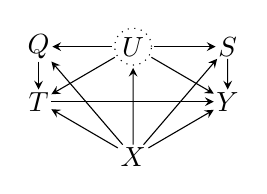
\begin{tikzpicture}[>=stealth,xscale=1.2,yscale=.7,inner sep=0pt,outer sep=1pt,baseline={(0,.3)}]
  \node[circle,draw,dotted,inner sep=1pt] (A) at (1,1) {$U$};
  \node (Q) at (0,1)  {$Q$};
  \node (S) at (2,1)  {$S$};
  \node (T) at (0,0)  {$T$};
  \node (Y) at (2,0)  {$Y$};
  \node (X) at (1,-1) {$X$};
  \draw[->] (A) -- (Q);
  \draw[->] (A) -- (S);
  \draw[->] (A) -- (T);
  \draw[->] (A) -- (Y);
  \draw[->] (Q) -- (T);
  \draw[->] (S) -- (Y);
  \draw[->] (T) -- (Y);
  \draw[->] (X) -- (T);
  \draw[->] (X) -- (Q);
  \draw[->] (X) -- (A);
  \draw[->] (X) -- (S);
  \draw[->] (X) -- (Y);
\end{tikzpicture}
\]

Here Q is a treatment-inducing proxy for U, and S an outcome-inducing
proxy. Under completeness conditions, there exists a ``bridge function''
$h(a,w)$ such that conditional expectations of $Y\mid T,Q$ can be
expressed as integrals of $h$ with respect to $S\mid T,Q$. The authors
construct neural estimators of these bridge functions and use them to
identify causal effects and evaluate policies in contextual bandits,
despite latent U.

\begin{center}\rule{0.5\linewidth}{0.5pt}\end{center}

\textbf{Causal inference using LLM-guided discovery}\\
A. Vashishtha et al.

Instead of asking an LLM for the entire DAG (which confounds direct and
indirect effects), they aim to recover only a \textbf{partial order}
compatible with the DAG. They use \textbf{triplet prompts}: given
(A,B,C), ask the model for the causal relations among them, and
aggregate across many triplets. From pairwise triplet votes they
reconstruct a partial order and compare it to a DAG via
\textbf{topological divergence} (number of edges incompatible with the
order).

This partial order can be used to:

\begin{itemize}
\tightlist
\item
  orient otherwise undirected edges in constraint-based algorithms (PC),
  or
\item
  constrain search in score-based methods (GES), e.g., by forbidding
  edges that violate the order.
\end{itemize}

\begin{center}\rule{0.5\linewidth}{0.5pt}\end{center}

\textbf{Causal order: the key to leveraging imperfect experts in causal
inference}\\
A. Vashishtha et al.~(2024)

Extends the above. They emphasize that pairwise LLM judgments (A causes
B or B causes A) are unreliable for distinguishing causation from common
causes and indirect effects. Triplet-based elicitation plus a focus on
ordering is more robust: it is easier for an expert (human or LLM) to
say which variables could be ``earlier'' causes without committing to
full graph structure. This gives useful constraints for choosing valid
adjustment sets or for orienting CPDAGs.

\begin{center}\rule{0.5\linewidth}{0.5pt}\end{center}

\subsection{Topic summary}\label{topic-summary-5}

The ``estimation'' and ``discovery'' halves of causality are finally
talking to each other. On the estimation side, double machine learning
has matured into a practical recipe: specify a low-dimensional estimand
(ATE, CATE, policy value), derive an orthogonal score, estimate all
nuisance functions flexibly, cross-fit, and then solve a simple
estimating equation. This removes much of the pain of choosing
parametric forms while retaining asymptotic theory. Brumback's R-centric
exposition brings this into routine practice: from basic DAGs and
backdoor sets to DiD, IV, mediation and time-varying confounding, with
sharper guidance on when each tool is valid.

At the same time, Xu et al.~show how proxy variables can rescue
identification even when key confounders are missing, at least under
strong completeness assumptions. Their neural bridge functions extend
ideas from proximal causal inference to bandits and high-dimensional
proxies.

On the discovery side, rather than treating LLMs as omniscient
DAG-oracles, Vashishtha et al.~advocate a humbler goal: learn only a
partial order on variables from triplet queries. Such an order is often
enough to choose safe adjustment sets (all ancestors of T that precede
Y) and to constrain or refine the output of PC/GES. This makes LLMs an
imperfect but usable source of causal \textbf{constraints}, rather than
an end-to-end solution.

\section{7. Graph learning, Laplacians, and Wasserstein
geometry}\label{graph-learning-laplacians-and-wasserstein-geometry}

\subsection{Papers}\label{papers-6}

\textbf{Optimization algorithms for graph Laplacian estimation via ADMM
and MM}\\
L. Zhao et al.

They consider estimation of a \textbf{combinatorial Laplacian} $L$ (zero
row-sum, nonpositive off-diagonal) from a sample covariance $S$, via
maximizing a Laplacian-structured Gaussian likelihood with $\ell^1$ sparsity:

\[
\begin{array}{ll}
\text{minimize}_L & \operatorname{tr}(LS) - \log\det^\ast L + \alpha\|L\|_{1,\mathrm{off}} \\
\text{s.t.} & L\mathbf{1}=0,\quad L_{ij}=L_{ji}\le0,\ L\succeq 0.
\end{array}
\]

Using $\det^\ast L$ (pseudo-determinant) is necessary because $L$ is
singular. They show that $\|L\|_1$ can be expressed as
$\operatorname{tr}(LH)$ for a fixed matrix $H$, and that passing to the reduced space via
the orthogonal complement of 1 simplifies the log-det term. They then
derive efficient ADMM and MM algorithms: ADMM for general sparsity, MM
for very sparse graphs. This provides a scalable way to estimate graph
structure and weights in Gaussian Markov random fields.

\begin{center}\rule{0.5\linewidth}{0.5pt}\end{center}

\textbf{Graphical models in heavy-tailed markets}\\
J.V. Cardoso et al.

Extends Laplacian-Gaussian MRFs to \textbf{heavy-tailed} financial
returns. Instead of assuming $(X\sim \mathcal{N}(0,\Sigma))$, they assume returns
are drawn from multivariate Student distributions or more general
elliptical models.

The generalized log-likelihood replaces the quadratic term $\operatorname{tr}(LS)$ by an
average of $\log\!\bigl(1 + x_i^\top L x_i/\nu\bigr)$, which yields robust estimation: large
deviations are downweighted. They also add a low-rank penalty
$\operatorname{tr}(V^\top L V)$ to encourage a limited number of connected
components (clusters) in the graph. This gives a Laplacian that reflects
both conditional independence and the heavy-tail structure of returns.

\begin{center}\rule{0.5\linewidth}{0.5pt}\end{center}

\textbf{Learning graphs from data} (your synthesis)

Your notes tie together several ideas:

\begin{itemize}
\tightlist
\item
  Treating graph learning as estimation of an adjacency or Laplacian
  matrix from smoothness assumptions: signals x should vary slowly over
  the graph, so minimize $\mathrm{tr}(XLX^\top) =
  \tfrac12\mathrm{tr}(WZ)$ where $Z$ encodes squared distances between
  samples.
\item
  Enforcing Laplacian constraints (row sums zero, nonpositive
  off-diagonals) and additional priors: degree regularization, target
  number of components via low-rank penalties $(\mathrm{tr}(F^\top L
  F))$, etc.
\item
  Robustifying to heavy-tailed data by replacing quadratic forms with
  $\log(1+\cdot)$ as in Student likelihoods.
\item
  Controlling connectivity and degrees (no isolated nodes) via
  constraints like $\operatorname{diag}(L)=1$ or $W\cdot \mathbf{1}=1$.
\end{itemize}

This framework unifies Laplacian graphical lasso, robust covariance
estimation, and structural priors on graphs.

\begin{center}\rule{0.5\linewidth}{0.5pt}\end{center}

\textbf{Spectral sparsification of graphs: theory and algorithms}\\
J. Batson et al.~(2009)\\
\textbf{Spectral sparsification of graphs}\\
D.A. Spielman and S.H. Teng (2010)

Spectral sparsifiers are sparse graphs that approximate the Laplacian
quadratic form of a dense graph:

\[ x^\top L_G x \approx x^\top L_{\tilde G} x\quad\forall x.
\]

Effective resistance $R_{uv}$ between nodes $u$ and $v$ quantifies how
crucial an edge is; sampling edges with probability proportional to
$w_{uv}R_{uv}$ and rescaling weights yields a near-optimal
sparsifier. Spielman and Teng develop nearly linear-time algorithms for
such sampling and show that a small number of random spanning trees also
produce good approximations. These tools give scalable approximations of
dense covariance or kernel graphs.

\begin{center}\rule{0.5\linewidth}{0.5pt}\end{center}

\textbf{Tree-sliced Wasserstein distance: a geometric perspective}\\
V.H. Tran et al.~(2025)

Instead of projecting distributions onto 1D lines (sliced Wasserstein),
tree-sliced Wasserstein (TSW) projects onto a \textbf{system of lines
organized by a tree}: lines intersect at nodes, but the tree is acyclic
so there is a unique path between any two points.

One constructs an arrangement of lines in $\mathbb{R}^d$, chooses a spanning tree on
the intersection graph, and defines a tree metric along these lines.
Probability measures are then projected onto this tree and compared via
1D Wasserstein distances along each branch. The result interpolates
between radial and directional projections and can approximate the true
Wasserstein distance with fewer projections, capturing global geometry
better.

\begin{center}\rule{0.5\linewidth}{0.5pt}\end{center}

\textbf{UltraTWD: optimizing ultrametric trees for tree-Wasserstein
distance}\\
F. Yu et al.~(2025)

Optimizes the \textbf{ultrametric} underlying a tree-Wasserstein
distance. An ultrametric can be represented as a rooted tree where all
leaves are equidistant from the root. They aim to find an ultrametric
distance $\tilde D$ that best approximates a given pairwise distance $D$,
under either $\ell^\infty$ or Frobenius norms.

For $\ell^\infty$, the optimal ultrametric can be extracted from the minimum
spanning tree (MST) of $D$ by a simple shift; for $\mathcal{F}$, the problem is
NP-hard but pseudo-convex and can be approximately solved via
gradient-based alternating optimization over node heights and tree
structure. Plugging these ultrametrics into tree-Wasserstein yields
effective distance measures with strong geometric structure.

\begin{center}\rule{0.5\linewidth}{0.5pt}\end{center}

\textbf{Tree-sliced variants of Wasserstein distances}\\
T. Le et al.~(2019)

Original TSW paper: proposes constructing random trees (quad trees,
hierarchical cluster trees) on data points, mapping distributions to
measures on tree nodes, and computing Wasserstein distances on these
trees. Sampling multiple random trees and averaging gives a
\textbf{tree-sliced Wasserstein} distance that is cheaper than full
Wasserstein and more informative than 1D slices.

\begin{center}\rule{0.5\linewidth}{0.5pt}\end{center}

\textbf{Lightspeed geometric dataset distance via sliced optimal
transport}\\
K. Nguyen et al.~(2025)

OTDD compares two datasets $(\mathcal{D}_1 = \{(x_i,y_i)\})$ and
$(\mathcal{D}_2=\{(x'_j,y'_j)\})$ by optimal transport over an
\textbf{augmented ground metric}:

\begin{itemize}
\tightlist
\item
  $d_X$ between features (e.g., Euclidean),
\item
  $d_Y$ between labels, defined via a distance between label-conditional
  feature distributions: \[ d_Y(y,y') =
  W_2\bigl(p(X\mid Y=y),p(X'\mid Y'=y')\bigr). \]
\end{itemize}

Originally $W_2$ between Gaussian approximations is used, but this is
costly. Lightspeed OTDD replaces this with \textbf{sliced distances}:
projecting features onto random lines, mapping these 1D distributions to
low-dimensional summary statistics (moments), and then computing
distances between those summaries. This drastically accelerates dataset
comparisons while preserving sensitivity to shifts in
label-conditionals.

\begin{center}\rule{0.5\linewidth}{0.5pt}\end{center}

\subsection{Topic summary}\label{topic-summary-6}

Graphs, Laplacians and optimal transport form a geometry of data. In
Gaussian models, the inverse covariance---or Laplacian in constrained
cases---is the object that encodes conditional independences. When
returns are heavy-tailed or exhibit clustered volatility, Gaussian
assumptions break; robust Laplacian estimators replace quadratic loss
with log(1+quadratic) terms and carry over sparsity and structural
constraints. The result is a graph that captures both dependence and
``risk flow'' in markets.

Spectral sparsification, via effective resistances or random spanning
trees, says that for many purposes you can replace a dense graph by a
much sparser one with almost the same quadratic form. This is
particularly appealing when graphs originate from dense covariance or
similarity matrices.

On the distributional side, the Wasserstein geometry is made cheaper and
more structured by slicing: along lines (classical sliced Wasserstein),
trees (tree-sliced), and now optimized ultrametrics (UltraTWD). Trees
and ultrametrics tie neatly back to hierarchical clustering and minimum
spanning trees. Lightspeed OTDD goes one step further: it defines a
notion of \textbf{distance between whole datasets} by mixing feature
distances with label-conditional distances, and makes it computationally
cheap using 1D projections.

Together, these tools provide a geometric view on both \textbf{network
structure} (through Laplacians) and \textbf{distribution comparison}
(through Wasserstein and its tree-based approximations), with direct
applications in portfolio construction, factor modeling, and data
selection.

\begin{center}\rule{0.5\linewidth}{0.5pt}\end{center}

\textsc{ChatGPT --}
\itshape
Next I'll move to:

\begin{itemize}
\tightlist
\item
  Portfolio optimization \& finance
\item
  Time series forecasting \& non-stationarity
\item
  Sparse / mechanistic interpretability
\item
  Diffusion \& continuous-time modeling
\item
  Bandits \& Bayesian optimization
\item
  Trees / rule ensembles / policy learning
\item
  Evaluation metrics \& change-points / clustering
\item
  Misc. optimization / operator-learning topics
\end{itemize}
\upshape

\textsc{ChatGPT --}
\itshape
Continuing.
\upshape

\section{8. Portfolio optimization, risk measures, and finance
applications}\label{portfolio-optimization-risk-measures-and-finance-applications}

\subsection{Books and general
frameworks}\label{books-and-general-frameworks}

\textbf{Portfolio optimization}\\
D.P. Palomar (2025)

Palomar's book is a modern, optimization-centric treatment of
portfolios. It covers:

\begin{itemize}
\tightlist
\item
  Stylized facts (non-stationarity, volatility clustering, fat tails,
  leverage, cross-sectional dependence).
\item
  Mean-variance and mean--risk formulations, with \textbf{fractional
  programs} for Sharpe and Kelly criteria. Fractional objectives are
  handled via bisection, Dinkelbach's transform, or Schaible's
  perspective transform, turning them into convex problems.
\item
  Shrinkage and robust estimation of means and covariances
  (James--Stein, Ledoit--Wolf, OAS, factor models, Black--Litterman),
  including random matrix pitfalls.
\item
  Time-series models (ARMA, GARCH, stochastic volatility, multivariate
  GARCH, DCC) and state-space models (Kalman filters) for volatility and
  correlation.
\item
  Graph-based portfolios: constructing MST / TMFG over correlations or
  learned Laplacians, then using hierarchical or Schur methods to
  combine assets and factors.
\item
  Risk measures beyond variance, including VaR, CVaR, EVaR, drawdowns,
  and spectral measures, with conic formulations (CVaR, EVaR) and
  scenario-based linearizations (MAD, CVaR).
\item
  Risk parity and risk budgeting portfolios (for variance and more
  general homogeneous risk measures), with convex and non-convex
  formulations and connections to eigenvalue problems.
\item
  Robust optimization (stochastic, chance-constrained, worst-case),
  including analytic centers and ``near-optimal centering'' to trade off
  point performance and robustness.
\end{itemize}

It's a very optimization-oriented view: most classical portfolio
problems are recast as convex or quasi-convex programs and solved by
interior point or SCA methods.

\begin{center}\rule{0.5\linewidth}{0.5pt}\end{center}

\textbf{Advanced portfolio optimization}\\
D. Cajas (2025)

Cajas's notes complement Palomar with:

\begin{itemize}
\item
  A survey of early work (Markowitz, CAPM, APT, risk parity,
  hierarchical risk parity, Kelly).
\item
  A catalogue of \textbf{risk measures} (coherent, convex, distortion,
  spectral, deviation, downside, range, drawdown, higher-moment,
  L-moments), including:

  \begin{itemize}
  \tightlist
  \item
    Spectral risk measures:
    \[ -\int q_X(u)\,\phi(u)\,du , \] with monotone
    weights $\phi(u)$.
  \item
    Entropic risk measures (EVaR):
    \[ \mathrm{EVaR}_\alpha(X)=\inf_{z>0}\frac{1}{z}\log \frac{\mathbb{E}[e^{X/z}]}{\alpha}. \]
  \item
    Relativistic VaR (RLVaR) based on $\kappa$-logarithms.
  \item
    Tail Gini and CVaR ranges.
  \end{itemize}
\item
  Constrained optimization formulations (including turnover, transaction
  costs, market impact, cardinality, minimum position sizes), often via
  mixed-integer programs or conic formulations.
\item
  Risk parity and hierarchical risk parity variants, including nested
  cluster optimization.
\item
  E/S-style and factor-based constraints represented as graph or factor
  penalties.
\end{itemize}

It's a dense ``catalogue of tricks'' for practitioners seeking to
express almost any portfolio desideratum as an optimization problem.

\begin{center}\rule{0.5\linewidth}{0.5pt}\end{center}

\textbf{Quantitative portfolio optimization: advanced techniques and
applications}\\
M. Noguer i Alonso et al.~(2025)

A collection of chapters on:

\begin{itemize}
\tightlist
\item
  Bayesian portfolios (including Black--Litterman, hierarchical priors,
  and Kalman filtering for dynamic portfolios).
\item
  Machine-learning-assisted allocations.
\item
  Factor models and nontraditional risk measures.
\item
  Case studies in equities, FX, and alternatives.
\end{itemize}

Your notes cover mainly the overlap with Palomar and Cajas; I'll
reference this as further reading rather than detail it.

\begin{center}\rule{0.5\linewidth}{0.5pt}\end{center}

\subsection{Relevance-based prediction and interpretable ``data
portfolios''}\label{relevance-based-prediction-and-interpretable-data-portfolios}

\textbf{Relevance}\\
M. Czasonis et al.~(2022)

OLS forecasts can be written as \textbf{relevance-weighted averages} of
past observations. For a new $x$, the linear predictor $\hat y =
x^\top \hat\beta$ can be rewritten as:

\[ \hat y = \bar y + \frac{1}{N-1}\sum_{i=1}^N r_i(x)\,(y_i-\bar y), \]

where the \textbf{relevance} $r_i(x)$ decomposes into:

\begin{itemize}
\tightlist
\item
  a similarity term:
  $-\tfrac12(x_i-x)^\top V^{-1}(x_i-x)$, i.e., minus
  Mahalanobis distance, and
\item
  an informativeness term: half the sum of informativeness of $x$ and
  $x_i$, measuring distance to the training mean.
\end{itemize}

Thus each training point is a ``mini model''; its weight in predicting $y$
for $x$ is an interpretable function of similarity and informativeness.

\begin{center}\rule{0.5\linewidth}{0.5pt}\end{center}

\textbf{Relevance-Based Prediction: a transparent and adaptive
alternative to machine learning}\\
M. Czasonis et al.~(2023)\\
\textbf{A Transparent Alternative to Neural Networks with an Application
to Predicting Volatility}\\
M. Czasonis et al.~(2024)\\
\textbf{The Virtue of Transparency: How to Maximize the Utility of Data
without Overfitting}\\
M. Czasonis et al.~(2024)

These papers build on the relevance representation:

\begin{itemize}
\item
  For each observation $x_t$, compute OLS-based relevance weights over
  the training set.
\item
  To improve robustness and interpretability, instead of using all
  training points, restrict to those with relevance above a threshold
  $r^*$, and rescale weights to preserve average leverage.
\item
  On a \textbf{grid} of relevance thresholds and variable subsets,
  compute ``partial-sample'' regressions and record:

  \begin{itemize}
  \tightlist
  \item
    Fit $R^2$,
  \item
    Asymmetry (difference between fit on high- vs low-relevance
    subsamples), and
  \item
    Adjusted fit = (\#variables) $\times$ (fit + asymmetry).
  \end{itemize}
\item
  Combine the corresponding models via adjusted-fit weights, like
  Bayesian model averaging but with a transparent model space (linear
  regressions with selected features and relevance cuts).
\end{itemize}

They argue this yields models that are as accurate as complex ML models
(e.g., for volatility prediction) but easier to audit: one can see which
past observations mattered, which features, and at what similarity
scale.

\begin{center}\rule{0.5\linewidth}{0.5pt}\end{center}

\textbf{A tale of tail covariances (and diversified tails)}\\
J. Rosensweig (2023)

Defines \textbf{tail covariances} as mixed odd moments such as
$\mathbb{E}[XY^{2k-1}]$ and $\mathbb{E}[X^{2k-1}Y]$,
which emphasize joint extreme moves rather than central behaviour.
Classical covariance is $k=1$; larger $k$ probe deeper into the tails. He
shows that portfolios that look diversified in variance may still be
highly concentrated in tail covariances, and proposes tail-covariance
analyses to assess ``tail diversification''.

\begin{center}\rule{0.5\linewidth}{0.5pt}\end{center}

\subsection{Risk measures and
drawdowns}\label{risk-measures-and-drawdowns}

\textbf{Properties of the entropic risk measure EVaR in relation to
selected distributions}\\
Y. Mishura et al.~(2024)

Studies EVaR for various parametric distributions and compares it to VaR
and CVaR. EVaR is coherent and often more conservative than CVaR,
especially in heavy-tailed settings. The paper gives explicit formulas
or approximations for EVaR under Gaussian and some non-Gaussian laws,
which is useful when plugging EVaR into optimization.

\begin{center}\rule{0.5\linewidth}{0.5pt}\end{center}

\textbf{Multistage stochastic programs with the entropic risk measure}\\
O. Dowson et al.

Formulates multistage decision problems (scenario trees) with EVaR as
risk measure. Using EVaR's exponential form, they derive tractable
convex programs (often via exponential cones) to optimize policies under
entropic risk constraints, analogous to CVaR-based multistage models but
with different sensitivity to tail shape.

\begin{center}\rule{0.5\linewidth}{0.5pt}\end{center}

\textbf{Constrained max drawdown: a fast and robust portfolio
optimization approach}\\
A. Dorador

Looks at \textbf{maximum drawdown (MDD)} as a risk constraint. Since
directly optimizing MDD is non-convex and involves all paths, the author
proposes approximations:

\begin{itemize}
\tightlist
\item
  Replace return variance with linear risk proxies (e.g., $\min_t
  \sum_i r_{it} w_i$) or absolute deviations).
\item
  Use mixed-integer formulations to enforce simple constraints on
  drawdown or on the number of assets.
\end{itemize}

Resulting linear or MILP formulations are practical and approximate
MDD-constrained portfolios reasonably well.

\begin{center}\rule{0.5\linewidth}{0.5pt}\end{center}

\subsection{Factor models, popularity, and
embeddings}\label{factor-models-popularity-and-embeddings}

\textbf{The popularity asset pricing model}\\
T.M. Idzorek et al.

Proposes a ``popularity'' explanation for many anomalies: investors
prefer certain assets (e.g., glamorous, ESG-friendly) beyond pure
risk-return trade-offs, generating persistent demand and excess returns
for unpopular assets. Popularity is not just taste: heterogeneity in
expectations also matters. Many so-called anomalies (value, low-vol,
etc.) can be reinterpreted as popularity premia.

\begin{center}\rule{0.5\linewidth}{0.5pt}\end{center}

\textbf{Domesticating the factor zoo with economic theory}\\
T.M. Idzorek et al.~(2024)

Extends the above. They argue that most of the ``factor zoo'' is better
seen as:

\begin{itemize}
\tightlist
\item
  A small number of \textbf{price factors} (risk/taste-driven,
  persistent premia), and
\item
  Many \textbf{attribution factors} (backward-looking decompositions of
  returns with zero unconditional premia).
\end{itemize}

A popularity-based equilibrium (PAPM) determines which factors belong to
which category. This offers an organizing principle to tame
proliferating factor lists.

\begin{center}\rule{0.5\linewidth}{0.5pt}\end{center}

\textbf{Asset embeddings}\\
X. Gabaix et al.~(2025)

Constructs asset embeddings from \textbf{holdings data} rather than
text:

\begin{itemize}
\tightlist
\item
  Recommender-style: log portfolio weights $ \log w_{ui}
  \approx \langle \phi_u,\phi_i\rangle$ where $u$ is an investor, $i$ an
  asset.
\item
  Word2vec/BERT-style: order assets in a portfolio by weight, treat them
  as ``sentences'', and learn context embeddings.
\end{itemize}

These embeddings correlate strongly with relative valuation and
co-movement structure, and are more informative than 10-K or
earnings-call embeddings for pricing and risk.

\begin{center}\rule{0.5\linewidth}{0.5pt}\end{center}

\subsection{Mean reversion, regimes, and learning to
rank}\label{mean-reversion-regimes-and-learning-to-rank}

\textbf{Identifying small mean-reverting portfolios}\\
A. d'Aspremont (2007)

Assumes prices follow a stationary VAR:

\[ S_t = A S_{t-1} + \varepsilon_t,\quad \Gamma =
\mathrm{Var}(S_t). \]

Mean reversion or predictability of a portfolio $p_t = w^\top S_t$ can be
quantified via:

\begin{itemize}
\tightlist
\item
  Autocorrelation $\beta$ = $\mathrm{cov}(p_t,p_{t-1}) / \mathrm{var}(p)$, or
\item
  Predictability $\nu =
  \dfrac{\mathrm{Var}(\hat p_t)}{\mathrm{Var}(p_t)}$.
\end{itemize}

Both can be expressed as \textbf{generalized Rayleigh quotients}:

\[ \lambda = 1 - \frac{w^\top A\Gamma w}{w^\top \Gamma w},\qquad \nu =
\frac{w^\top A\Gamma A^\top w}{w^\top \Gamma w}. \]

Finding sparse portfolios $w$ that minimize $\nu$ (or maximize mean reversion)
becomes a sparse generalized eigenvalue problem, solvable by greedy
search, brute force (for small sets), or SDP relaxations.

\begin{center}\rule{0.5\linewidth}{0.5pt}\end{center}

\textbf{Regime-aware factor allocation with optimal feature selection}\\
T. Bosancic et al.~(2025)

Uses \textbf{jump models} to detect regimes in factor and macro data:
cluster time points into K states $s_t$ and regime means $\theta_k$ while
penalizing changes in state:

\[ \min \sum_t |y_t - \theta_{s_t}|^2 +
\lambda \sum_t \mathbf{1}\{s_t\neq s_{t-1}\}, \]

or a relaxed version with $s_t$ on the simplex and fused-lasso penalties.
These are extended with sparse feature selection (à la sparse k-means),
and applied to factor returns (value, size, profitability) and macro
variables (PE, DP, S\&P, etc.) to define ``durable'' vs ``fragile''
regimes. Allocation switches between factor exposures and T-bills
depending on the regime.

\begin{center}\rule{0.5\linewidth}{0.5pt}\end{center}

\textbf{Learning hidden Markov models with persistent states by
penalizing jumps (jump models)}\\
P. Nystrup et al.~(2020) and follow-ups

The \textbf{jump model} formulation is equivalent to an HMM with a
penalty on state changes; dynamic programming can solve for $s_t$ given
$\theta_k$, and vice versa. Continuous extensions put $s_t$ on the simplex and
penalize $\| s_t-s_{t-1}\|_1^2$, yielding soft
regimes. Nystrup et al.~and Aydinḥan et al.~apply these to financial
time series, combining with sparse feature selection to find
interpretable regime-driving variables.

\begin{center}\rule{0.5\linewidth}{0.5pt}\end{center}

\textbf{Enhancing long-short portfolios: a refined approach using
learning to rank algorithms}\\
M. Linger et al.

Portfolio construction is often a 2-step process: predict scores, then
form long--short portfolios based on ranks. Learning-to-rank (LTR)
models (pairwise or listwise losses: RankNet, ListNet, ListMLE) can be
trained directly to rank assets by future returns. The paper designs
\textbf{tail-sensitive} ranking losses that care most about correct
ordering near the long and short extremes, e.g.~weighted ListMLE or
ListFold focusing on extreme pairs. These produce better long--short
strategies than regressing returns and then sorting.

\begin{center}\rule{0.5\linewidth}{0.5pt}\end{center}

\subsection{Interpretability and tree-based models in
finance}\label{interpretability-and-treebased-models-in-finance}

\textbf{Interpretable supervised portfolios}\\
G. Chevalier et al.

The ``supervised portfolio'' approach forecasts \textbf{optimal weights}
(e.g., ex-post Sharpe-optimal) as a function of features. Chevalier et
al.~use \textbf{RuleFit} to make such maps interpretable: train boosted
trees, extract path-based rules, then fit an $\ell^1$-penalized linear model
in both original features and rule indicators. The result is a sparse
set of human-readable rules for weight adjustments, preserving much of
the performance of black-box models.

\begin{center}\rule{0.5\linewidth}{0.5pt}\end{center}

\textbf{Predictive learning via rule ensembles (RuleFit)}\\
J.H. Friedman and B.E. Popescu (2008)

RuleFit in general: fit a tree ensemble, extract rules (root-to-leaf
paths), standardize rule activations and original features, and fit an
$\ell^1$-penalized linear model. This yields additive models combining linear
main effects and sparse, interpretable interactions.

\begin{center}\rule{0.5\linewidth}{0.5pt}\end{center}

\textbf{Node Harvest}\\
N. Meinshausen (2010)

Rather than combining indicator rules, NodeHarvest works with node
predictions: every internal/leaf node of a forest predicts an outcome;
the final prediction is a convex combination of these node means.
Weights are learned so that predictions remain interpretable as averages
over human-readable subgroups.

\begin{center}\rule{0.5\linewidth}{0.5pt}\end{center}

\textbf{SIRUS: Interpretable random forests via rule extraction}\\
C. Bénard et al.

SIRUS trains a random forest with shallow, quantile-split trees,
extracts frequent rules, removes redundant ones, and fits a ridge
regression on rule activations. The resulting models are stable (small
changes in data do not change rules much) and interpretable; they apply
naturally to score-based or weight-based portfolio models.

\begin{center}\rule{0.5\linewidth}{0.5pt}\end{center}

\textbf{RIPE: Rule induction partitioning estimator}\\
V. Margot et al.

RIPE builds a set of low-dimensional axis-aligned rules
(hyperrectangles), and defines predictions for a point $x$ based on the
intersection of all rules containing $x$ minus the union of rules not
containing $x$. This yields a non-tree partition; the final rule set is
pruned via empirical risk minimization, yielding yet another
interpretable alternative to deep nets.

\begin{center}\rule{0.5\linewidth}{0.5pt}\end{center}

\textbf{The adaptive lasso and its oracle properties}\\
H. Zou (2006)

Adaptive lasso applies variable-adaptive $\ell^1$ penalties, e.g.
\begin{align*}
  \hat\beta &= \operatorname*{Argmin}_\beta \|y - X\beta\|_2^2 +
  \lambda\sum_i w_i\,|\beta_i|
  \\
  w_i &=
  \frac{1}{|\hat\beta^{\text{(initial)}}_i|}.
\end{align*}
Sparse models whose small coefficients are penalized more strongly can
achieve oracle properties (correct variable selection + asymptotic
normality) under conditions. This is useful when combining many rules or
features (RuleFit, RIPE).

\begin{center}\rule{0.5\linewidth}{0.5pt}\end{center}

\subsection{Miscellaneous finance
applications}\label{miscellaneous-finance-applications}

\textbf{Dual interpretation of machine learning forecasts}\\
P. Goulet Colombe et al.

Shows that forecasts of many ML models (ridge, kernel ridge, nets,
random forests, boosting) can be written as \textbf{linear combinations
of training labels}:
\[ \hat y_j = \sum_{i\in \text{Train}} w_{ij}\, y_i. \]
These weights can be interpreted as a ``data portfolio'' for each test
point. The authors propose diagnostics such as contributions
$c_{ij}=w_{ij}y_i$, weight concentration, negative-weight mass,
total weight, turnover $\| w_{\cdot j}-w_{\cdot, j-1}\|_1$, and historical importance
$\| w_{i\cdot}\|_1$. This dual view aids interpretability
and debugging of learned strategies.

\begin{center}\rule{0.5\linewidth}{0.5pt}\end{center}

\textbf{In-sample and out-of-sample Sharpe ratios for linear predictive
models}\\
A. Jacquier et al.~(2025)

In a Gaussian linear model $r_{t+1} = \beta s_t +
\varepsilon_{t+1}$, with $s_t$ as signals and returns multivariate
normal, they derive the distribution of in-sample and out-of-sample
Sharpe ratios for Markowitz portfolios constructed from the signals. In
particular, they quantify the bias of in-sample Sharpe as an estimator
of true performance, offering corrections and confidence intervals for
strategies built via linear prediction.

\begin{center}\rule{0.5\linewidth}{0.5pt}\end{center}

\textbf{Regimes}\\
A. Mulliner et al.~(2025)

A simple regime approach:

\begin{itemize}
\tightlist
\item
  Select a small set of macro/market variables (S\&P 500, term spreads,
  short rates, oil, copper, VIX, stock--bond correlation).
\item
  Measure Euclidean similarity between today's state and the historical
  states.
\item
  Examine subsequent returns of assets that historically out- or
  under-performed in similar environments.
\end{itemize}

Invest accordingly, or use the most dissimilar environments to invert
the historical strategy. Your note suggests Mahalanobis distance (and
learned metrics) improve this slightly but at the cost of overfitting.

\begin{center}\rule{0.5\linewidth}{0.5pt}\end{center}

\textbf{RiskMiner: discovering formulaic alphas via risk-seeking Monte
Carlo tree search}\\
T. Ren et al.

(Not detailed here earlier, but your notes mention it under RL \&
finance.) RiskMiner frames alpha search as a Monte Carlo tree search
over symbolic expressions, using a \textbf{risk-seeking} RL objective
(e.g., quantiles of cumulative reward) rather than expected reward. It's
a modern alternative to genetic programming for ``alpha mining''.

\begin{center}\rule{0.5\linewidth}{0.5pt}\end{center}

\subsection{Topic summary}\label{topic-summary-7}

The classical portfolio problems---mean--variance, Sharpe asymptotics,
factor models---are now surrounded by a ring of more nuanced questions:
What exactly counts as risk? How do we avoid overfitting? How do we keep
models interpretable?

Palomar, Cajas and Noguer i Alonso provide the formal machinery: almost
any notion of risk (variance, CVaR, drawdowns, entropic measures, tail
Gini, ranges) has a convex or mixed-integer representation; almost any
constraint (turnover, lot sizes, regimes) can be expressed as a cone or
a few integers. On top of this, modern kernels and shrinkage produce
better inputs (covariances and forecasts), and random matrix theory
warns us about the limits of eigen-omniscience.

Czasonis et al.~take a different route: instead of adding more layers of
nonlinearity, they re-express OLS as relevance-weighted averages of past
data, and then build ensembles of partial-sample models along a
``relevance grid''. The result looks like a very old idea---an average
of simple regressions---but with a principled way to choose and weight
them. When combined with diagnostics like the deflated Sharpe ratio and
Jacquier's Sharpe corrections, this kind of transparent modelling makes
it harder to p-hack oneself.

Finally, factor and regime stories are being re-examined. Popularity,
tail covariances and asset embeddings give new ways to think about risk
premia and co-movement, while jump models and learning-to-rank losses
offer more realistic ways to decide when, and on whom, to bet.

\begin{center}\rule{0.5\linewidth}{0.5pt}\end{center}

\textsc{ChatGPT --}
\itshape
Due to length, I'll stop here. Remaining topics to cover (in the same
way):

\begin{itemize}
\tightlist
\item
  Time series forecasting \& non-stationarity
\item
  Sparse / mechanistic interpretability
\item
  Diffusion \& continuous-time modeling
\item
  Bandits \& Bayesian optimization
\item
  Trees / rule ensembles / policy learning (more general, outside
  finance)
\item
  Evaluation metrics \& change-points / clustering
\item
  Misc. optimization / operator-learning topics
\end{itemize}
\upshape

\textsc{ChatGPT --}
\itshape
Continuing.
\upshape

\section{9. Time series forecasting and
non-stationarity}\label{time-series-forecasting-and-nonstationarity}

\subsection{Normalization and
non-stationarity}\label{normalization-and-nonstationarity}

\textbf{TimeBridge: non-stationarity matters for long-term time series
forecasting}\\
P. Liu et al.~(2025)

TimeBridge addresses the tension between removing non-stationarity (to
stabilize relationships) and preserving it (to capture long-term
structure and cointegration). It splits series into patches, embeds them
via per-series MLPs, and processes them through several attention blocks
that each see different normalizations:

\begin{itemize}
\tightlist
\item
  \textbf{Stationary attention}: patch embeddings minus moving averages
  (remove low-frequency drift).
\item
  \textbf{Downsampled attention}: attention between coarse-grained
  patches to model slow trends.
\item
  \textbf{Cointegrated attention}: attention on raw patches to retain
  long-run dependencies.
\end{itemize}

Each attention block is followed by two LayerNorm+MLP sublayers.
Combining these ``views'' yields better long-term forecasts on
non-stationary data than models that normalize everything the same way.

\begin{center}\rule{0.5\linewidth}{0.5pt}\end{center}

\textbf{Reversible instance normalization for accurate time-series
forecasting against distribution shift (RevIN)}\\
T. Kim et al.

RevIN applies a learnable per-instance affine normalization before
forecasting, then inverts it:

\[ \hat x_{it} =
\gamma\cdot \frac{x_{it} - \mathbb{E}_i[x_{it}]}{\sqrt{\mathrm{Var}_i[x_{it}] + \epsilon}}
+ \beta. \]

This operation is applied to the input series so that the forecasting
model sees approximately stationary data. The parameters $\gamma,\beta$ are
learned, so the normalization can adapt to the task. After forecasting,
the inverse transform maps predictions back to the original scale. RevIN
is simple but very effective for domain shifts where the mean and
variance of series (across time or across domains) differ.

\begin{center}\rule{0.5\linewidth}{0.5pt}\end{center}

\textbf{Dish-TS: a general paradigm for alleviating distribution shift
in time series forecasting}\\
W. Fan et al.

Dish-TS generalizes RevIN: it learns separate normalization and
de-normalization transforms of the form

\[ \tilde x = \frac{x - \mu_\theta(x)}{\sigma_\theta(x)}, \]

where $\mu$ and $\sigma$ are neural networks. Input and output transforms can
differ, handling shifts not only in level and scale but also in more
complex forms. The forecasting model sits between these transforms. This
``distribution shift'' sandwich is designed to handle covariate and
label shifts between training and deployment time.

\begin{center}\rule{0.5\linewidth}{0.5pt}\end{center}

\textbf{Adaptive normalization for non-stationary time series
forecasting: a temporal slice perspective}\\
Z. Liu et al.

This method slices time along windows and applies adaptive
normalizations per slice. Different time slices (e.g., recent vs
long-ago) can receive different affine maps, learned jointly with the
forecasting network. This better captures non-stationarity that changes
over time rather than being constant across the dataset.

\begin{center}\rule{0.5\linewidth}{0.5pt}\end{center}

\textbf{Non-stationary diffusion for probabilistic time series
forecasting}\\
W. Ye et al.

Diffusion-based TS forecasters usually assume \textbf{homoskedastic}
noise (additive Gaussian). Ye et al.~propose a \textbf{location--scale}
noise model:

\[ Y = f_\phi(X) +
\sqrt{g_\psi(X)}\,\varepsilon,\quad \varepsilon\sim \mathcal{N}(0,I), \]

where both mean and conditional variance $g_\psi(X)$ are learned. They
integrate this into a diffusion model where the noise schedule and the
denoising network respect conditional heteroskedasticity, leading to
better calibrated probabilistic forecasts.

\begin{center}\rule{0.5\linewidth}{0.5pt}\end{center}

\textbf{KoNODE: Koopman-driven neural ordinary differential equations
with evolving parameters for time series analysis}\\
H. Bai and W. Ding

KoNODE extends neural ODEs for time series. A neural ODE models dynamics
as $\dot x = f(x,t,\theta)$ with fixed parameters $\theta$. KoNODE allows $\theta$
itself to evolve according to a linear dynamical system:

\[ \theta_t = h(w_t),\quad \dot w_t = A w_t. \]

So while dynamics are nonlinear in $x$, the evolution of parameters is
linear in a lifted state space $w$. This is conceptually a Koopman
operator on parameters. It can capture non-stationary dynamics where the
underlying ODE slowly changes over time.

\begin{center}\rule{0.5\linewidth}{0.5pt}\end{center}

\subsection{Time-series foundation models and
evaluation}\label{time-series-foundation-models-and-evaluation}

\textbf{Time-series foundation model for value-at-risk}\\
A. Goel et al.~(2024)

Explores using \textbf{pretrained time-series foundation models} (e.g.,
TimeFM) for VaR estimation. After fine-tuning, these models are
competitive with econometric baselines (GARCH, GAS), especially when
data are scarce or multi-scale. They provide flexible, data-driven
predictive distributions rather than single-quantile models.

\begin{center}\rule{0.5\linewidth}{0.5pt}\end{center}

\textbf{Topical works from last year}\\
(MOMENT, Lag-Llama, decoder-only TS foundation models; Time-LLM, One
Fits All)

Your previous notes already covered attempts to port transformer LLMs to
time series (via patch embeddings, frequency-domain transformers,
reprogramming text models). This year's readings reinforce the sense
that while these models are flexible, simpler AR or N-BEATS-type
baselines remain surprisingly competitive.

\begin{center}\rule{0.5\linewidth}{0.5pt}\end{center}

\textbf{Cik: Context is key -- a benchmark for forecasting with
essential textual information}\\
A.R. Williams et al.

Cik is a benchmark for \textbf{multimodal} time-series forecasting where
each time series is accompanied by \textbf{essential text context}
(e.g., descriptions, events). Models must forecast using both numeric
and textual information. The authors provide evaluation metrics like
CRPS, and a variant RCRPS (region-of-interest CRPS) that emphasizes
particular forecast horizons and constraints. This pushes toward TS
models that leverage news, descriptions, or sensor metadata.

\begin{center}\rule{0.5\linewidth}{0.5pt}\end{center}

\textbf{Forecast evaluation for data scientists: common pitfalls and
best practices}\\
H. Hewamalage et al.

A survey of error and scoring metrics for TS forecasting. Emphasizes:

\begin{itemize}
\tightlist
\item
  Always compare to simple baselines (naïve, seasonal naïve).
\item
  Be wary of non-stationarity, seasonality, heteroskedasticity and
  structural breaks when choosing metrics.
\item
  For probabilistic forecasts, use \textbf{proper scoring rules} such as
  CRPS or log-likelihood; account for dimensionality (energy scores can
  be misleading).
\item
  Avoid data leakage via improper cross-validation (e.g., rolling vs
  shuffling).
\end{itemize}

It is a practical companion to the more theoretical probabilistic
modelling papers.

\begin{center}\rule{0.5\linewidth}{0.5pt}\end{center}

\textbf{Chronos: learning the language of time series}\\
A.F. Ansari et al.

Chronos treats time series like text by:

\begin{itemize}
\tightlist
\item
  Mean-scaling and \textbf{quantizing} values into discrete tokens.
\item
  Training a T5-style transformer to predict future tokens
  autoregressively.
\item
  Enhancing training data via \textbf{TSMixup} and \textbf{KernelSynth}
  (Gaussian process--based synthetic series).
\end{itemize}

The model outputs full predictive distributions over future quantized
values and can be fine-tuned to downstream tasks (forecasting, anomaly
detection).

\begin{center}\rule{0.5\linewidth}{0.5pt}\end{center}

\textbf{The effectiveness of discretization in forecasting: an empirical
study on neural time series models}\\
S. Rabanset et al.

Systematically studies discretizing time series (value binning) before
feeding them to deep models (MLPs, CNNs, RNNs). Finds that quantization
often \textbf{improves} performance, likely because it reduces noise and
stabilizes gradients. This supports the discretize-then-transformer
approach of Chronos and similar models.

\begin{center}\rule{0.5\linewidth}{0.5pt}\end{center}

\textbf{Maximum entropy bootstrap for time series: the meboot R
package}\\
H.D. Vinod and J. López-de-Lacalle

Describes the \textbf{maximum entropy bootstrap} for TS, which:

\begin{enumerate}
\def\labelenumi{\arabic{enumi}.}
\tightlist
\item
  Separates the order of observations from their values.
\item
  Fits a piecewise maximum-entropy distribution consistent with the data
  (e.g., matching means on intervals).
\item
  Resamples values from this distribution while preserving the original
  order.
\end{enumerate}

Unlike block bootstrap or stationary bootstrap, it aims to respect
non-stationarity and avoid underrepresenting extremes. Useful for
bootstrap-based inference on TS (e.g., for Sharpe ratios or regression
coefficients).

\begin{center}\rule{0.5\linewidth}{0.5pt}\end{center}

\textbf{The uncertainty of machine learning predictions in asset
pricing}\\
Y. Liao et al.~(2025)

For panel data and deep predictors of returns, they propose a
\textbf{wild bootstrap} variant:

\begin{itemize}
\tightlist
\item
  Fit a model $\hat y_{it}$ on returns $r_{it}$.
\item
  Compute residuals $\varepsilon_{it}$.
\item
  For each bootstrap, sample a common $\eta_t\sim \mathcal{N}(0,1)$ across assets
  (preserving cross-sectional dependence) and set $r^*_{it} =
  \hat y_{it} + \eta_t \varepsilon_{it}$.
\item
  Fine-tune the model for a few epochs and recompute predictions.
\end{itemize}

This yields bootstrap ensembles from which prediction intervals can be
computed. They then propose worst-case portfolio optimization using
these intervals (optimize under the worst plausible return vector in a
conformal/bootstrapped sense).

\begin{center}\rule{0.5\linewidth}{0.5pt}\end{center}

\subsection{Topic summary}\label{topic-summary-8}

Time-series forecasting is slowly absorbing the lesson that
non-stationarity is the rule, not the exception. Normalization
tricks---RevIN, Dish-TS, slice-wise normalization---can be seen as
learned, input-dependent stationarizers: they strip away some of the
drift and scale variation before giving the data to a model, then
re-insert it after forecasting. TimeBridge explicitly separates
stationary and non-stationary components at the patch level and lets
different attention mechanisms deal with them.

On the probabilistic side, diffusion models and
discretize-then-transformer models like Chronos are starting to compete
with traditional econometric approaches. But their usefulness depends on
how we \textbf{evaluate} them: Hewamalage's tutorial and the Cik
benchmark remind us that metrics matter---a poor CRPS or miscalibrated
quantiles can make complex models useless in risk-sensitive settings.

Finally, the bootstrap is alive and well, just more sophisticated.
Maximum entropy bootstraps acknowledge that financial series are rarely
stationary; wild residual bootstraps that share shocks across assets
respect cross-sectional dependence. When combined with TS foundation
models, these tools promise more honest uncertainty quantification than
a lone GARCH fit or a single neural network run.

\begin{center}\rule{0.5\linewidth}{0.5pt}\end{center}

\textsc{ChatGPT --}
\itshape
Given the length, I'll pause again. Remaining topics:

\begin{itemize}
\tightlist
\item
  Sparse / mechanistic interpretability
\item
  Diffusion \& continuous-time modeling
\item
  Bandits \& Bayesian optimization
\item
  Trees / rule ensembles / general policy learning
\item
  Evaluation metrics \& change-points / clustering
\item
  Misc. optimization / operator-learning topics
\end{itemize}
\upshape

\textsc{ChatGPT --}
\itshape
Continuing.
\upshape

\section{10. Sparse / mechanistic interpretability and
SAEs}\label{sparse-mechanistic-interpretability-and-saes}

\subsection{Sparse autoencoders and feature
circuits}\label{sparse-autoencoders-and-feature-circuits}

\textbf{Scaling monosemanticity: extracting interpretable features from
Claude 3 Sonnet}\\
A. Templeton et al.

Anthropic train large \textbf{sparse autoencoders} (SAEs) on activations
of Claude 3 Sonnet to obtain monosemantic features: each latent ideally
corresponds to a single human-interpretable concept. These SAEs are
overcomplete (more features than neurons) but enforced to be sparse and
roughly nonnegative; activations live in a high-dimensional feature
space where specific units track sentiments, topics, syntax, or
safety-relevant behaviours (e.g.~deception, weapons). They show that
many such features can be labeled with short textual descriptions and
that manipulating them (e.g.~ablating ``deception'' features) reliably
changes model behaviour.

The work is both a scaling story (SAEs over dozens of layers) and an
interpretability demonstration: you can browse features in an
interactive UMAP and check their top activating tokens and contexts.

\begin{center}\rule{0.5\linewidth}{0.5pt}\end{center}

\textbf{Gemma Scope: open sparse autoencoders everywhere all at once on
Gemma 2}\\
T. Lieberum et al.

Extends SAE analysis to Google's Gemma-2. They train SAEs over:

\begin{itemize}
\tightlist
\item
  MLP activations, and
\item
  Residual stream activations,
\end{itemize}

for many layers, using ReLU or JumpReLU and top-k sparsity. They find
thousands of interpretable features (e.g.~country names, HTML tags,
refusal patterns), confirm that many neurons are polysemantic, and show
that SAEs quite effectively disentangle them. The open release of models
and tooling makes Gemma a convenient playground for mechanistic
interpretability.

\begin{center}\rule{0.5\linewidth}{0.5pt}\end{center}

\textbf{Jumping ahead: improving reconstruction fidelity with JumpReLU
sparse autoencoders}\\
S. Rajamanoharan et al.

Standard SAEs use ReLU with $L^1$ penalties, which introduce shrinkage and
often yield many near-zero but not exactly zero activations. JumpReLU
introduces a trainable threshold $\theta$ and defines

\[ \sigma(z) = \mathrm{JumpReLU}_\theta(z) = z\,\mathbf{1}_{\{z\ge \theta\}}, \]

which is exactly zero below $\theta$ and linear above. They train with
straight-through gradient estimators for the step and handle $\ell^0$ sparsity
by using the count of preactivations above $\theta$. JumpReLU SAEs achieve
better reconstruction at a given sparsity level and more clearly
``on/off'' features.

\begin{center}\rule{0.5\linewidth}{0.5pt}\end{center}

\textbf{Improving dictionary learning with gated sparse autoencoders}\\
S. Rajamanoharan et al.

Gated SAEs split feature selection (gates) from value prediction:
\begin{align*}
  g &= W_0 x + b_0 \\
   y &=
  \mathbf{1}_{g\ge 0}\odot \mathrm{ReLU}(W_1 x + b_1)
  \\
   \hat x &=
W_2 y + b_2,
\end{align*}
with a relation between $W_0$ and $W_1$ so that the gate controls whether a
feature is used while a second linear map sets its magnitude. This
reduces shrinkage bias and helps avoid dead units. Gated SAEs can learn
cleaner, more stable dictionaries.

\begin{center}\rule{0.5\linewidth}{0.5pt}\end{center}

\textbf{Scaling and evaluating sparse autoencoders}\\
L. Gao et al.

A systematic study of design choices for SAEs on LLMs:

\begin{itemize}
\tightlist
\item
  \textbf{Top-k activation} (or MultiTopK) instead of $L^1$ penalties to
  enforce exact sparsity.
\item
  Initialize decoder $W_2$ as the transpose of encoder $W_1$.
\item
  Add an \textbf{auxiliary loss} that reconstructs inputs from
  normally-dead units, to keep more features alive.
\end{itemize}

They also propose MultiTopK losses combining several $k$ (e.g.~$\ell_k + \tfrac{1}{8}\,\ell_{4k}$)
so that features remain informative at multiple sparsity levels and can
be used flexibly at test time. These tricks significantly improve
reconstruction and interpretability of learned features.

\begin{center}\rule{0.5\linewidth}{0.5pt}\end{center}

\textbf{Learning multi-level features with Matryoshka sparse
autoencoders}\\
B. Bussmann et al.

Matryoshka SAEs enforce that the first m features alone reconstruct the
input well, for multiple $m\in\mathcal{M}$ (e.g., 64, 128, 256, \ldots). They minimize
a \textbf{sum of losses over prefix lengths}:

\[ \ell = \sum_{m\in\mathcal{M}} \| x - f_m(x) \|_2^2 + \alpha\,\ell_{\text{aux}}. \]

This encourages a hierarchy: early features capture broad, high-level
structure; later ones add refinements. They also explore different
sparsifiers: JumpReLU, Top-k, BatchTopK, and show that Matryoshka
constraints stabilize features across scales and help avoid ``feature
splitting'' where high-level features fracture into many low-level ones.

\begin{center}\rule{0.5\linewidth}{0.5pt}\end{center}

\textbf{Universal sparse autoencoders: interpretable cross-model concept
alignment}\\
H. Thasarathan et al.

Instead of training separate SAEs for each model, Universal SAEs are
trained on activations from \textbf{multiple pretrained models} (e.g.,
different vision or language architectures) simultaneously. Shared
latent units are thus encouraged to represent concepts that are common
across models. Each model has its own encoder/decoder head into the
shared latent space. This yields cross-model aligned features and
enables cross-model editing: attenuating a concept in one model based on
concept directions learned jointly.

\begin{center}\rule{0.5\linewidth}{0.5pt}\end{center}

\textbf{Transcoders find interpretable LLM feature circuits}\\
J. Dunefsky et al.

A \textbf{transcoder} approximates the dense MLP at a layer with a
wider, sparse MLP:

\[ z = \mathrm{ReLU}(W_1 x + b_1),\quad \hat y = W_2 z + b_2, \]

but trained to match the original MLP's output $y$. The idea is to
represent the original layer as a composition of many sparse
monosemantic units. Once trained, one can:

\begin{itemize}
\tightlist
\item
  Identify important units for a behaviour,
\item
  Extract small ``circuits'' (paths through the transcoder) that
  reproduce that behaviour, and
\item
  Modify or remove them.
\end{itemize}

They propose greedy methods to build sparse subgraphs (feature circuits)
that track a specific capability (e.g., subject--verb agreement).

\begin{center}\rule{0.5\linewidth}{0.5pt}\end{center}

\textbf{Sparse feature circuits: discovering and editing interpretable
causal graphs in language models}\\
S. Marks et al.

Builds on SAEs and transcoders to discover \textbf{feature circuits}:
small, sparse subgraphs of the model responsible for particular
behaviours. They show:

\begin{itemize}
\tightlist
\item
  Many such circuits can be discovered and labeled (e.g.~``gender
  bias'', ``refusal'', ``in-character persona'').
\item
  Editing them (by ablating or rescaling features) has predictable
  causal effects on model outputs.
\end{itemize}

This provides a more robust concept-level handle on models than shallow
prompt engineering.

\begin{center}\rule{0.5\linewidth}{0.5pt}\end{center}

\subsection{Interpretable attributions and local
explanations}\label{interpretable-attributions-and-local-explanations}

\textbf{AttnLRP: Attention-aware layer-wise relevance propagation for
transformers}\\
R. Achtibat et al.

Extends \textbf{Layer-Wise Relevance Propagation (LRP)} to transformers.
Key issues are treating attention (multiplicative, masked, with softmax)
and layernorm in a way consistent with LRP's ``relevance conservation''.
AttnLRP linearizes attention blocks and propagates relevance through
queries, keys and values, yielding token-level attributions that respect
the model's structure. Implemented in the \texttt{lxt} library, it allows
detailed inspection of which input tokens contribute most to a given
prediction in transformer models.

\begin{center}\rule{0.5\linewidth}{0.5pt}\end{center}

\textbf{Local rule-based explanations of black box decision systems
(LoRE)}\\
R. Guidotti et al.

LoRE is a model-agnostic local explainer. For a point $x$, it:

\begin{enumerate}
\def\labelenumi{\arabic{enumi}.}
\tightlist
\item
  Generates a synthetic neighbourhood around $x$ (with a genetic algorithm
  that seeks informative perturbations near the decision boundary).
\item
  Trains a decision tree approximating the black box locally.
\item
  Extracts a rule describing $x$'s decision and proposes counterfactuals:
  minimal rule changes that flip the predicted label.
\end{enumerate}

Unlike LIME, which uses linear models, LoRE's trees capture local
nonlinearities while remaining human-readable.

\begin{center}\rule{0.5\linewidth}{0.5pt}\end{center}

\textbf{Explaining nonlinear classification decisions with deep Taylor
decomposition}\\
G. Montavon et al.

Deep Taylor decomposition explains $f(x)$ by distributing its value back
to input features via local Taylor expansions around suitable root
points. For each neuron or layer, they consider the mapping to its
relevance $R$ (instead of output) and expand around a point where $R$ is
zero. This yields relevance propagation rules reminiscent of LRP but
grounded in Taylor theory. For RELU nets with box-constrained inputs,
they derive simple closed-form decompositions that satisfy positivity
and conservation of relevance.

\begin{center}\rule{0.5\linewidth}{0.5pt}\end{center}

\subsection{Topic summary}\label{topic-summary-9}

Mechanistic interpretability is converging on a small set of core tools:
sparse autoencoders to discover monosemantic features, transcoders to
re-express dense computations as sums of sparse ones, and attribution
methods to trace which parts of input and network matter for a given
behaviour.

SAEs are now applied at scale (Claude, Gemma), across many layers, and
even across models. Variants like JumpReLU, gated SAEs, and Matryoshka
constraints improve reconstruction, avoid dead units and encourage
multi-level hierarchies. The result is a growing dictionary of
human-readable features: from tokens and syntactic roles to political
leanings, deception patterns and safety-relevant content. Transcoders
and sparse feature circuits then allow those features to be stitched
into small directed graphs that behave like ``cognitive subroutines''
inside the LLM.

On the explanation side, LRP and deep Taylor decomposition generalise
smoothly to transformers via AttnLRP; local rule-based explainers like
LoRE give human-digestible descriptions and counterfactuals around
individual inputs. All of this is still young, but compared to even two
years ago, we now have concrete, working tools to ask not just
\emph{what} models predict, but \emph{which internal features and
circuits} they use.

\section{11. Diffusion, continuous-time flows, and Schrödinger
bridges}\label{diffusion-continuous-time-flows-and-schruxf6dinger-bridges}

\subsection{Continuous-time generative models and rectified
flows}\label{continuous-time-generative-models-and-rectified-flows}

\textbf{Continuous time generative models}\\
(Q. Liu, ICML 2025 tutorial)

This tutorial unifies flows, diffusions and resampling schemes. Given
two distributions $p_0, p_1$, we want a transport process $Z_t$ such that
$Z_0\sim p_0$ and $Z_1\sim p_1$. The classical optimal transport (OT) problem minimizes
an integral of a cost c along trajectories, but OT paths can be curved
and hard to parametrize. For generative modelling, we prefer
\textbf{straight paths}: they require fewer steps and simpler dynamics.

Enter \textbf{rectified flows}: start with an easy coupling ($X_0\sim p_0$,
$X_1\sim p_1$ independent), define the linear interpolation

\[ X_t = (1-t)X_0 + t X_1,\quad \dot X_t = X_1-X_0, \]

and then learn a velocity field $v_t(x)\approx \mathbb{E}[\dot X_t \mid X_t = x]$.
This yields an ODE that transports $p_0$ to $p_1$ along approximately straight
paths. One can iterate this procedure: after learning v, regenerate a
coupling using the new map, and refine. Under mild assumptions,
rectification reduces curvature while preserving marginals and decreases
transport cost for any convex path cost.

The tutorial also:

\begin{itemize}
\tightlist
\item
  Relates flows and diffusions via Fokker--Planck: an SDE and its
  associated ODE have the same marginals but different sample paths.
\item
  Shows how to incorporate constraints (e.g., manifold support $\Omega$ or
  discrete supports) via \textbf{$\Omega$-bridges} or deterministic correction
  forces.
\item
  Derives relationships between velocity fields, data scores $\nabla \log \rho_t$
  and denoising; Tweedie's formula connects rectified flows to
  score-based diffusion.
\end{itemize}

\begin{center}\rule{0.5\linewidth}{0.5pt}\end{center}

\textbf{Harnessing low dimensionality in diffusion models}\\
(ICML 2025 tutorial)

Diffusion models are surprisingly \textbf{reproducible}: two models
trained independently on the same dataset produce strikingly similar
outputs when seeded with the same noise. At the same time, they
\textbf{generalize} correctly when trained on sufficiently large
datasets: their samples differ significantly from training data, and the
fraction of samples close (e.g., via SSCD similarity) to any training
point is small.

The key link is the intrinsic dimension of data. For a dataset,
intrinsic dimension m can be estimated from k-NN distances $T_k(x)$ via

\[ \hat m_k(x) =
\left(\frac{1}{k-1}\sum_{j=1}^{k-1}\log \frac{T_k(x)}{T_j(x)}\right)^{-1}.
\]

ImageNet, for example, has intrinsic dimension $\approx 40$--$50$. Diffusion models
trained on $N$ samples with latent dimension $\gg m$ can approximate the data
distribution well once $N\ge (L/\varepsilon)^m$. In that regime, both
reproducibility (two models learning the same manifold) and
generalization (new samples far from training points) become expected.
Conversely, small datasets lead to memorization.

The tutorial also shows that many architectures implicitly reduce data
to a low-dimensional manifold inside the high-dimensional noise space,
and that understanding this manifold is crucial for assessing privacy
leakage and memorization.

\begin{center}\rule{0.5\linewidth}{0.5pt}\end{center}

\textbf{Mini-works referenced last year}\\
(Karras et al.~on design space, Lipman et al.~on flow matching, Albergo
et al.~on stochastic interpolants, Xu et al.~on Poisson flows, Song \&
Dhariwal on consistency models)

Your new readings build on those: rectified flows and consistency models
are extensions of the notion that flows and diffusions can be combined
and unified, and that different choices of forward process and training
target (noise, score, velocity) yield different trade-offs.

\begin{center}\rule{0.5\linewidth}{0.5pt}\end{center}

\subsection{Action matching and Schrödinger
bridges}\label{action-matching-and-schruxf6dinger-bridges}

\textbf{Action matching: learning stochastic dynamics from samples}\\
K. Neklyudov et al.

Given a stochastic process $X_t$, the \textbf{rectified flow} defines a
deterministic flow with the same one-time marginals by setting
$v_t(x)=\mathbb{E}[\dot X_t \mid X_t=x]$. Action Matching leverages this to
fit \textbf{reverse-time SDEs} and flows. They consider the functional
\begin{align*}
  \mathcal{L}_\mathrm{AM}(s) = {}& \mathbb{E}[s_0(X_0)] +
\mathbb{E}[s_1(X_1)] + \\
& \int_0^1
\mathbb{E}\left[\tfrac12\|v_t(X_t)\|^2 + \partial_t s_t(X_t)\right] dt,
\end{align*}
where s are ``actions'' whose gradient gives the flow. Minimizing this
functional recovers dynamics that match the marginals and approximate
pathwise properties of $X_t$. They extend this to Schrödinger bridges
(minimum-KL couplings to Brownian motion) and unbalanced transport,
giving a family of methods to learn dynamics consistent with
intermediate marginals and end constraints.

\begin{center}\rule{0.5\linewidth}{0.5pt}\end{center}

\textbf{Trajectory inference with smooth Schrödinger bridges}\\
W. Hong et al.~(2025)

Classic Schrödinger bridges compare stochastic processes by minimizing
KL to a reference Brownian motion subject to endpoint constraints. Hong
et al.~consider replacing Brownian motion with \textbf{smooth Gaussian
processes} (e.g.~Matérn), better suited to modelling smooth dynamics.
They derive algorithms to estimate these bridges and apply them to
interpolate between observed endpoints in noisy dynamical systems.
Compared to Brownian-bridge-based methods, the resulting trajectories
are smoother and more realistic.

\begin{center}\rule{0.5\linewidth}{0.5pt}\end{center}

\textbf{Designing losses for data-free training of normalizing flows on
Boltzmann distributions}\\
L. Felardos et al.

Flows are often trained via maximum likelihood, which requires
evaluating target densities up to a normalizing constant. For
\textbf{Boltzmann distributions} $p(x)\propto e^{-E(x)}$, they propose
training flows without data by minimizing the variance of importance
weights:

\[ \operatorname*{Var}_{x\sim q_\theta}
\Bigl[\log \frac{p(x)}{q_\theta(x)}\Bigr], \]

with $p(x)$ given only through unnormalized energies. They derive losses
based on log-sum-exp and demonstrate that minimizing the variance of
log-weights leads the flow to match $p$. This is useful in statistical
physics and Bayesian inverse problems, where $p$ is expensive but data
samples are unavailable.

\begin{center}\rule{0.5\linewidth}{0.5pt}\end{center}

\textbf{Neural relational inference for interacting systems}\\
T. Kipf et al.~(2018)

(Not new this year, but referenced in your notes.) Neural Relational
Inference uses graph neural networks to infer latent interaction graphs
between particles from observed trajectories. It uses a variational
graph encoder to propose edges and a decoder that simulates dynamics
given the graph. It fits nicely into the ``dynamics + structure''
picture where we combine generative models of trajectories with learnt
latent graphs.

\begin{center}\rule{0.5\linewidth}{0.5pt}\end{center}

\subsection{Topic summary}\label{topic-summary-10}

Diffusion models began as glorified denoisers; they are quickly turning
into a general language for probabilistic dynamics. Rectified flows and
action matching connect them to optimal transport and control: rather
than following wiggly Brownian paths, we learn straight or nearly
straight ODEs whose marginals match the data. Schrödinger bridges
connect those ODEs back to SDEs, expressing a preference for certain
base processes (Brownian, Matérn) and adding a ``path prior'' to the
family of generative models.

The picture that emerges is that of \textbf{data manifolds in noise
space}, evolving under time-dependent velocity fields. Intrinsic
dimension estimates help explain when diffusion models generalize vs
memorize; sliced and tree-sliced Wasserstein measures tell us how far
apart distributions really are. For finance and physics, where both path
details and tail behaviour matter, these tools provide a richer and more
controllable framework than GANs or naive flows.

\section{12. Bandits, off-policy evaluation, and Bayesian
optimization}\label{bandits-off-policy-evaluation-and-bayesian-optimization}

\subsection{Contextual bandits and
exploration}\label{contextual-bandits-and-exploration}

\textbf{A contextual bandit approach to personalized news article
recommendation}\\
L. Li et al.~(2010)

Introduces \textbf{LinUCB} for contextual bandits: rewards are assumed
linear in context $x$ with parameter $\theta$, and we maintain a ridge regression
posterior $(A, b)$. The UCB index for arm i is

\[ \mathrm{UCB}_i = x_i^\top \hat\theta +
\alpha\sqrt{x_i^\top A^{-1}x_i}, \]

where $(\hat\theta=A^{-1}b)$. LinUCB has provable regret bounds and
works well in news recommendation, where each article has contextual
features. The paper also proposes a \textbf{hybrid LinUCB} where some
features are shared across arms and some are arm-specific.

\begin{center}\rule{0.5\linewidth}{0.5pt}\end{center}

\textbf{Thompson sampling for contextual bandits with linear payoffs
(LinTS)}\\
S. Agrawal and N. Goyal (2013)

Extends Thompson sampling to linear contextual bandits by maintaining a
Bayesian posterior over $\theta$ (Gaussian with mean and covariance from linear
regression) and sampling $\bar\theta$ from that posterior at each round, then
choosing the arm maximizing $x_i^\top \bar\theta$. LinTS is conceptually parallel to
LinUCB but uses randomization rather than upper confidence bounds, and
enjoys similar regret guarantees.

\begin{center}\rule{0.5\linewidth}{0.5pt}\end{center}

\textbf{Value-difference based exploration: adaptive control between
epsilon-greedy and softmax}\\
M. Tokic and G. Palm

Value-difference exploration dynamically tunes between $\varepsilon$-greedy and
softmax. When value estimates for the top arms are close (high
uncertainty), it behaves more like softmax (more exploration); when one
arm is clearly better, it behaves more like greedy. This adaptively
balances exploration and exploitation without a pre-fixed schedule.

\begin{center}\rule{0.5\linewidth}{0.5pt}\end{center}

\textbf{Algorithms for the multi-armed bandit problem}\\
V. Kuleshov and D. Precup (survey)

Covers a range of bandit algorithms:

\begin{itemize}
\tightlist
\item
  $\varepsilon$-greedy, softmax, pursuit methods.
\item
  UCB variants (UCB1, UCB-V, etc.).
\item
  Exp3/Exp4 for adversarial bandits.
\item
  Contextual extensions and regret bounds.
\end{itemize}

Useful as background for understanding the contextual methods above.

\begin{center}\rule{0.5\linewidth}{0.5pt}\end{center}

\textbf{Dynamic clustering of contextual multi-armed bandits}\\
T.T. Nguyen and H.W. Lauw (2014)

DynUCB introduces \textbf{clustered LinUCB}:

\begin{itemize}
\tightlist
\item
  Fit a LinUCB model for each user.
\item
  Periodically cluster the user parameter vectors with k-means.
\item
  For each user, use a mixture (or cluster centroid) model to compute
  LinUCB indices.
\end{itemize}

This allows sharing statistical strength across similar users while
preserving some personalization. It's an early example of joint
representation learning and bandit policies.

\begin{center}\rule{0.5\linewidth}{0.5pt}\end{center}

\textbf{Nonparametric bandits with covariates}\\
P. Rigollet and A. Zeevi (2018)

Studies contextual bandits with arbitrary (nonlinear) reward functions
of context. A simple strategy---grid the context space and run a
separate UCB in each cell---achieves sublinear regret, but only
polynomial rates are possible in the worst case. The paper provides
lower bounds showing that high-dimensional, smooth nonlinear bandits
inherently suffer from curse-of-dimensionality in regret.

\begin{center}\rule{0.5\linewidth}{0.5pt}\end{center}

\textbf{Nonparametric stochastic contextual bandits}\\
M.Y. Guan and H. Jiang (2018)

Proposes \textbf{k-NN-UCB}: for a context x, find its k nearest
neighbours, estimate rewards locally, and apply UCB using the local
sample size. Under Lipschitz assumptions, this achieves sublinear regret
and can adapt to local structures better than global linear models.

\begin{center}\rule{0.5\linewidth}{0.5pt}\end{center}

\textbf{A practical method for solving contextual bandit problems using
decision trees}\\
A.N. Elmachtoub et al.

Uses decision trees as base learners in contextual bandits, combined
with \textbf{bootstrap Thompson sampling}:

\begin{itemize}
\tightlist
\item
  Fit a tree model $f$ to predict rewards from contexts.
\item
  For Thompson sampling, fit several trees on bootstrap resamples of the
  data and, at each round, randomly pick one tree and choose the arm
  with best predicted reward.
\end{itemize}

This gives a Bayesian-like sampling scheme without explicit posterior
distributions, leveraging tree variance for exploration.

\begin{center}\rule{0.5\linewidth}{0.5pt}\end{center}

\textbf{The epoch-greedy algorithm for contextual multi-armed bandits}\\
J. Langford and T. Zhang

Epoch-greedy interleaves exploration and exploitation:

\begin{enumerate}
\def\labelenumi{\arabic{enumi}.}
\tightlist
\item
  In \textbf{exploration} steps, pick arms uniformly at random and
  collect data.
\item
  After enough exploration, in \textbf{exploitation} steps, choose arms
  according to the best policy in a finite policy class, as estimated
  from the exploration data.
\end{enumerate}

Exploration lengths are chosen based on regret bounds for the best
policy in the class. This gives finite-sample guarantees when the policy
class is known and finite (e.g., linear threshold rules).

\begin{center}\rule{0.5\linewidth}{0.5pt}\end{center}

\subsection{Off-policy evaluation and
influence}\label{off-policy-evaluation-and-influence}

\textbf{Doubly robust policy evaluation and optimization}\\
M. Dudík et al.~(2014)

Doubly robust (DR) estimators combine a \textbf{direct method} (outcome
model) and \textbf{IPW} (propensity model):

\[ \hat V_\mathrm{DR}(\pi) = \frac1n\sum_{i=1}^n \bigl[
\hat\mu_{\pi(X_i)}(X_i) +
\frac{\mathbf{1}_{T_i=\pi(X_i)}}{\hat e(T_i|X_i)} (Y_i - \hat\mu_{T_i}(X_i))
\bigr]. \]

If either the propensity model or the outcome model is correct (not
necessarily both), the estimator is consistent. Dudík et al.~show that
DR estimators have lower variance than IPW alone and can be used within
\textbf{policy search}: optimize over $\pi$ to maximize
$\hat V_\mathrm{DR}(\pi)$ while controlling complexity.

\begin{center}\rule{0.5\linewidth}{0.5pt}\end{center}

\textbf{Open Bandit Dataset and Pipeline: towards realistic and
reproducible off-policy valuation}\\
Y. Saito et al.~(2021)

OpenBandit provides real contextual bandit data (e-commerce
recommendations) with known logging policies, allowing benchmarking of
OPE methods (DM, IPW, SNIPW, DR, switch estimators, DR-with-shrinkage,
etc.). They implement many methods and show that \textbf{self-normalized
IPW} and \textbf{shrinkage DR} variants strike favourable bias--variance
trade-offs. This is an important benchmark for bandit off-policy
evaluation in realistic settings.

\begin{center}\rule{0.5\linewidth}{0.5pt}\end{center}

\textbf{Log-sum-exponential estimator for off-policy evaluation and
learning}\\
(Your summary)

Proposes LSE-based mean estimators for heavy-tailed returns:
\[ \mathrm{LSE}_\lambda(z_1,\dots,z_n) =
\frac1\lambda \log\left(\frac1n\sum_i e^{\lambda z_i}\right). \]

Applied to OPE, $z_i$ can be importance-weighted rewards. For appropriate
$\lambda$, the LSE estimator has lower variance and better MSE than plain
averages, especially when importance weights are heavy-tailed.

\begin{center}\rule{0.5\linewidth}{0.5pt}\end{center}

\textbf{Outlier gradient analysis: efficiently identifying detrimental
training samples for deep learning}\\
A. Chhabra et al.~(2025)

Given a trained deep model, they embed per-sample gradients into a
``gradient space'' and use outlier detection (e.g., isolation forests)
there. Samples whose gradients are highly atypical are candidates for
\textbf{detrimental training points}, analogous to negative influence in
influence functions. Unlike classical influence that relies on Hessian
inversion, this method is cheap and scales to modern nets.

\begin{center}\rule{0.5\linewidth}{0.5pt}\end{center}

\textbf{Understanding black-box predictions via influence functions}\\
P.W. Koh and P. Liang (2017)

Influence functions approximate the effect of upweighting or removing a
training point $z_j$ on parameters $\hat\theta$ and downstream losses via:
\[ I(z_j) =
-H^{-1}\nabla_\theta \ell(z_j,\hat\theta), \]
where $H$ is the Hessian of the empirical loss. They use this to:

\begin{itemize}
\tightlist
\item
  Identify training points most responsible for a given prediction.
\item
  Construct upweighting approximations of leave-one-out risk.
\item
  Build adversarial training points.
\end{itemize}

In deep nets, exact Hessian inversion is infeasible, but LiSSA and
Hessian--vector products allow approximations.

\begin{center}\rule{0.5\linewidth}{0.5pt}\end{center}

\textbf{Second-order stochastic optimization for machine learning in
linear time}\\
N. Agarwal et al.~(2017)

Introduces LiSSA, which approximates $H^{-1}v$ by expanding $H^{-1}$ as a Neumann
series:

\[ H^{-1} = (I - (I-H))^{-1} =
\sum_{k=0}^\infty (I-H)^k, \]

and replacing $H$ by unbiased stochastic estimates $\nabla^2 f_i$.
This gives a cheap approximation to influence directions and Newton
updates in large-scale settings.

\begin{center}\rule{0.5\linewidth}{0.5pt}\end{center}

\textbf{On second-order group influence functions for black-box
predictions}\\
S. Basu et al.~(2020)

Individual influence approximations can be loose when many training
points jointly affect a prediction. Group influence replaces single $z$ by
sets $U$, computing second-order expansions to better capture interactions
within $U$. This is applicable in settings like dataset distillation and
causal auditing of data subsets.

\begin{center}\rule{0.5\linewidth}{0.5pt}\end{center}

\textbf{Discriminative Jackknife: quantifying uncertainty in deep
learning via higher-order influence functions}\\
A.M. Alaa and M. van der Schaar (2020)

Combines influence functions with \textbf{Jackknife} ideas to build
predictive intervals around deep net predictions. For each training
point, approximate the effect of leaving it out via influence functions;
aggregate to obtain variance estimates for predictions, and calibrate
them via higher-order corrections. They propose intervals that do not
require retraining the network.

\begin{center}\rule{0.5\linewidth}{0.5pt}\end{center}

\textbf{Beta Shapley: a unified and noise-reduced data valuation
framework for machine learning}\\
Y. Kwon and J. Zou

Data Shapley values average each point's marginal contribution over all
dataset sizes; this is high-variance and expensive. Beta Shapley
replaces the uniform over sizes with a Beta($\alpha,\beta$) prior,
emphasizing either small ($\alpha<1$, $\beta=1$) or large ($\alpha=1$, $\beta<1$)
coalitions. This preserves desirable Shapley axioms, yields a family of
valuations (from leave-one-out--like to full-dataset--like), and reduces
variance.

\begin{center}\rule{0.5\linewidth}{0.5pt}\end{center}

\textbf{DataInf: efficiently estimating data influence in LoRA-tuned
LLMs and diffusion models}\\
Y. Kwon et al.

To compute influence in large models, they approximate the Hessian $H$ by
the \textbf{Fisher information} (outer products of gradients) and
block-diagonalize it per layer. For each block, they further approximate
$H^{-1}$ with either:

\begin{itemize}
\tightlist
\item
  Rank-k Empirical Fisher inverses (using Sherman--Morrison on rank-1
  updates), or
\item
  Swapping expectation and inversion to simplify.
\end{itemize}

This reduces computation of $H^{-1}v$ drastically, enabling approximate
influence analysis in LoRA-tuned LLMs and diffusion models.

\begin{center}\rule{0.5\linewidth}{0.5pt}\end{center}

\subsection{Bayesian optimization}\label{bayesian-optimization}

\textbf{Earl-NO: reinforcement learning for multi-step lookahead,
high-dimensional Bayesian optimization}\\
M. Cheon et al.

Standard Bayesian optimization (BO) typically uses \textbf{one-step
lookahead} acquisition functions (EI, UCB). Earl-NO formulates
multi-step lookahead BO as an RL problem:

\begin{itemize}
\tightlist
\item
  State: a set of past queried points and outcomes, embedded by DeepSets
  and Transformers.
\item
  Action: a new point to evaluate.
\item
  Reward: improvement in best value, possibly discounted.
\end{itemize}

They train a PPO agent to optimize these rewards on synthetic BO tasks
and then apply it to high-dimensional BO problems. Earl-NO learns
\textbf{policies} that implicitly account for multi-step consequences,
going beyond myopic BO.

\begin{center}\rule{0.5\linewidth}{0.5pt}\end{center}

\textbf{Understanding high-dimensional Bayesian optimization}\\
L. Papenmeier et al.~(2025)

Survey of techniques for high-dimensional BO:

\begin{itemize}
\tightlist
\item
  Random embeddings to low-dimensional subspaces.
\item
  Additive or axis-aligned assumptions on the objective.
\item
  Local BO (e.g.~CMA-ES-like local search framed as BO).
\item
  Lengthscale priors scaled with dimension.
\end{itemize}

They argue that no single approach works universally; structural
assumptions about the objective (additivity, sparsity,
low-effective-dimension) are crucial.

\begin{center}\rule{0.5\linewidth}{0.5pt}\end{center}

\subsection{Topic summary}\label{topic-summary-11}

Bandits and BO illustrate two faces of ``learning under limited
feedback'': bandits make decisions sequentially with partial rewards, BO
optimizes black-box functions with few evaluations. The toolbox is now
rich: LinUCB and LinTS for linear structure, k-NN and trees for
nonparametric structure, DynUCB for clustered users, epoch-greedy for
finite policy classes. On top of that, DR estimators and OPE benchmarks
like OpenBandit show how to evaluate new policies from logged data
without running fresh experiments.

Under the hood, influence functions and their modern approximations
(LiSSA, DataInf) provide a way to track how each datapoint affects a
model's decisions, and how reliable those decisions are. They form a
bridge between purely algorithmic regret bounds and the practical
question ``which data should I trust or keep?''---a question central to
both bandits and portfolio applications.

On the BO side, the trend mirrors that in TS and causal discovery: from
carefully engineered myopic criteria to learned \textbf{policies} that
treat the optimization itself as an RL problem. The cost is higher
complexity; the reward is better global exploration in high dimensions
when the right structural assumptions (sparsity, low effective
dimension) hold.

\begin{center}\rule{0.5\linewidth}{0.5pt}\end{center}

\textsc{ChatGPT --}
\itshape
Given the length, I'll stop here. Remaining topics:

\begin{itemize}
\tightlist
\item
  Trees / rule ensembles / policy learning (beyond finance)
\item
  Evaluation metrics \& change-points / clustering
\item
  Miscellaneous optimization / operator-learning topics
\end{itemize}

If you'd like, I can proceed to those next, then we'll be done with step
3.
\upshape

\textsc{ChatGPT --}
\itshape
Continuing.
\upshape

\section{13. Trees, rule ensembles, and policy learning (beyond
finance)}\label{trees-rule-ensembles-and-policy-learning-beyond-finance}

\subsection{Optimal and model-based
trees}\label{optimal-and-model-based-trees}

\textbf{Optimal classification trees}\\
D. Bertsimas and J. Dunn (2015)

Standard decision trees (CART) are grown greedily and pruned; they are
not globally optimal. Bertsimas and Dunn formulate tree induction as a
\textbf{mixed-integer program}:

\begin{itemize}
\tightlist
\item
  Binary variables for whether an internal node splits.
\item
  Binary variables to choose the splitting feature at each node.
\item
  Constraints linking sample assignments, feature tests, and leaf
  labels.
\end{itemize}

The objective is to minimize misclassification (or a surrogate) plus a
complexity penalty. Warm starts from CART and progressive deepening
(increasing maximum depth, node counts) make the MIP feasible for
moderate-sized problems. The approach extends to regression and
multivariate trees.

\begin{center}\rule{0.5\linewidth}{0.5pt}\end{center}

\textbf{Learning optimal and fair decision trees for non-discriminative
decision-making}\\
S. Aghaei et al.

Generalizes optimal trees to \textbf{fairness-constrained} settings.
They adapt the MIP formulation to incorporate:

\begin{itemize}
\tightlist
\item
  Group fairness constraints (e.g., equal error rates across protected
  groups), and
\item
  Fairness penalties in the objective.
\end{itemize}

The constraints are linearizable, so the resulting MIPs remain solvable
with modern solvers. This yields trees that trade off accuracy and
fairness in a controlled, global way.

\begin{center}\rule{0.5\linewidth}{0.5pt}\end{center}

\textbf{Learning optimal classification trees using a binary linear
program formulation}\\
S. Verwer and Y. Zhang

Refines the MIP by aggregating constraints over rows with the same
feature patterns, reducing the number of constraints from $O(n)$ to the
number of distinct input patterns. This often leads to significant
speedups without changing the global optimum.

\begin{center}\rule{0.5\linewidth}{0.5pt}\end{center}

\textbf{Optimal constraint-based decision tree induction from itemset
lattices}\\
S. Nijssen and E. Fromont

DL8 is an \textbf{exhaustive search} tree learner for binary data that
uses frequent itemset mining. Each path from root to leaf corresponds to
an itemset; the algorithm:

\begin{itemize}
\tightlist
\item
  Explores the itemset lattice,
\item
  Prunes subtrees using upper bounds on attainable accuracy, and
\item
  Guarantees optimal trees under given constraints (max depth, min
  support).
\end{itemize}

It is especially suited to high-dimensional, sparse, binary features.

\begin{center}\rule{0.5\linewidth}{0.5pt}\end{center}

\textbf{Learning optimal decision trees using caching branch-and-bound
search (DL8.5)}\\
G. Aglin et al.

DL8.5 improves DL8 with caching and more aggressive bounding.
Subproblems (subsets of examples) and their optimal subtrees are cached;
branch-and-bound prunes unpromising branches. The PyDL8.5 implementation
is considerably faster than standard MIP formulations for many problems.

\begin{center}\rule{0.5\linewidth}{0.5pt}\end{center}

\textbf{Node Harvest}\\
N. Meinshausen (2010) -- already mentioned under portfolios

In a more general ML context, NodeHarvest uses nodes from a random
forest as building blocks and learns non-negative weights over them so
that predictions are convex combinations of node means. This provides
global interpretability (each node is a hyper-rectangle with its own
mean), robustness, and handles continuous targets as well as
classification.

\begin{center}\rule{0.5\linewidth}{0.5pt}\end{center}

\textbf{ctree and MOB: model-based trees}\\
T. Hothorn et al.~-- ``ctree: conditional inference trees''\\
A. Zeileis and T. Hothorn -- ``Parties, models, mobsters''

Model-based recursive partitioning (MOB) builds trees where each leaf
contains a \textbf{parametric model}, not just a constant. The splitting
is guided by \textbf{parameter instability tests}:

\begin{enumerate}
\def\labelenumi{\arabic{enumi}.}
\tightlist
\item
  Fit a model (e.g., linear regression) $Y\sim g(X;\theta)$ in the current node.
\item
  Test whether residuals or score contributions depend on candidate
  splitters $Z$ (supLM tests, fluctuation tests à la Zeileis \& Hornik).
\item
  If significant instability is detected for some $Z$, split on $Z$ and
  refit models in children.
\end{enumerate}

\texttt{ctree} (conditional inference trees) similarly uses hypothesis tests
(e.g.~permutation tests of independence) to choose splits, avoiding
biased split selection. These methods provide trees that are less prone
to overfitting and allow arbitrary parametric models in leaves.

\begin{center}\rule{0.5\linewidth}{0.5pt}\end{center}

\textbf{Ckmeans.1d.dp: optimal k-means clustering in one dimension by
dynamic programming}\\
H. Wang and M. Song

While not a tree per se, this 1D dynamic programming algorithm for
$k$-means is used in many contexts (e.g.~for binning targets or features).
It computes the exact optimal partition into $k$ segments in O(kn) time,
and is implemented in R's \texttt{Ckmeans.1d.dp} package.

\begin{center}\rule{0.5\linewidth}{0.5pt}\end{center}

\subsection{Policy trees, prescriptive trees, and
bandits}\label{policy-trees-prescriptive-trees-and-bandits}

\textbf{Optimal policy trees}\\
M. Amram et al.

Policy trees partition covariate space and assign treatments in each
leaf. Amram et al.~formulate \textbf{policy learning} as a MIP using
doubly robust estimates of counterfactual outcomes:

\begin{enumerate}
\def\labelenumi{\arabic{enumi}.}
\tightlist
\item
  Estimate potential outcomes $\hat Y(0,X)$, $\hat Y(1,X)$ and
  propensity scores $e(X)$.
\item
  Construct DR pseudo-outcomes $\Gamma_{it}$ for each treatment $t$.
\item
  Build a tree whose leaves assign treatments to maximize accumulated $\Gamma$
  (or minimize cost), subject to tree complexity constraints.
\end{enumerate}

This yields globally optimal treatment policies of bounded depth and
complexity.

\begin{center}\rule{0.5\linewidth}{0.5pt}\end{center}

\textbf{Optimal prescriptive trees}\\
D. Bertsimas et al.

Tackles the joint problem of:

\begin{itemize}
\tightlist
\item
  Learning counterfactual models (possibly piecewise linear in leaves),
  and
\item
  Learning an optimal treatment policy tree.
\end{itemize}

The algorithm alternates between fitting leaf models and optimizing
splits via MIPs, directly targeting a prescriptive objective (e.g.,
expected profit or expected utility). It generalizes policy trees beyond
constant-leaf models.

\begin{center}\rule{0.5\linewidth}{0.5pt}\end{center}

\textbf{evtree: evolutionary learning of globally optimal classification
and regression trees in R}\\
T. Grubinger et al.~(2014)

evtree uses an \textbf{evolutionary algorithm} to search tree space.
Candidate trees undergo mutation (changing splits, swapping subtrees)
and crossover, with fitness based on predictive performance and
complexity. This avoids solving large MIPs and can approximate globally
optimal trees when exact methods are too expensive.

\begin{center}\rule{0.5\linewidth}{0.5pt}\end{center}

\textbf{Approximation trees: statistical stability in model
distillation}\\
Y. Zhou et al.

Approximation trees distill a black-box model (e.g., a random forest)
into a decision tree that is both accurate and statistically
\textbf{stable}. They:

\begin{itemize}
\tightlist
\item
  Fit a tree on pseudo-observations (x, f(x)+noise), where noise
  promotes exploration near the decision boundary.
\item
  Use statistical tests on the Gini index to prune and choose the depth
  and number of pseudo-samples so that splits are likely to be stable
  across resamples.
\end{itemize}

This balances fidelity to the black-box with interpretability and
robustness.

\begin{center}\rule{0.5\linewidth}{0.5pt}\end{center}

\textbf{Decision tree induction through LLMs via semantically-aware
evolution}\\
T. Liu et al.

Uses LLMs as mutation operators in an evolutionary algorithm for
decision trees:

\begin{itemize}
\tightlist
\item
  Maintain a population of trees.
\item
  For mutation, prompt the LLM with problem context, existing trees and
  their fitness, and ask it to propose new trees that are different,
  more interpretable or higher-performing.
\end{itemize}

The LLM thus provides semantically meaningful modifications, not just
random perturbations. This approach leverages language understanding to
guide the search in tree space.

\begin{center}\rule{0.5\linewidth}{0.5pt}\end{center}

\subsection{Topic summary}\label{topic-summary-12}

Decision trees, in their classical greedy form, are easy to interpret
but notoriously suboptimal. The last decade has produced multiple ways
to escape this limitation:

\begin{itemize}
\tightlist
\item
  \textbf{MIP-based exact trees} (Bertsimas \& Dunn, Aghaei et al.,
  Verwer \& Zhang) guarantee optimality under rich constraints,
  including fairness.
\item
  \textbf{Itemset-based search} (DL8.5) leverages frequent patterns to
  constrain the search.
\item
  \textbf{Model-based trees} (ctree, MOB) integrate parametric models
  and statistical tests into the splitting criterion.
\end{itemize}

On top of that, policy trees extend the idea to decision making: each
leaf prescribes an action, chosen to maximize doubly robust estimates of
treatment effect. Approximation trees and LLM-guided evolution close the
loop: they take a complex black-box or a prior population of trees and
iteratively refine interpretable surrogates.

The picture is that of a \textbf{continuum between trees as models and
trees as policies}, with optimization and modern statistical theory
ensuring that interpretability is no longer synonymous with mediocrity.

\section{14. Evaluation metrics, clustering comparison, and
change-point
detection}\label{evaluation-metrics-clustering-comparison-and-change-point-detection}

\subsection{Clustering and community detection
metrics}\label{clustering-and-community-detection-metrics}

\textbf{Information theoretic measures for clusterings comparison:
variants, properties, normalization and correction for chance}\\
N.X. Vinh et al.

Reviews measures like mutual information (MI), normalized mutual
information (NMI), adjusted Rand index, and proposes the
\textbf{normalized information distance}:

\[ \mathrm{NID}(U,V) = 1 - \frac{I(U;V)}{\max{H(U),H(V)}}. \]

To correct for chance (random clusterings with the same cluster sizes),
they suggest subtracting the expected index under random partitions and
rescaling:

\[
\frac{\text{index}-\mathbb{E}[\text{index}]}{\max(\text{index})-\mathbb{E}[\text{index}]}.
\]

This improves interpretability and comparability across tasks with
different numbers of clusters or classes.

\begin{center}\rule{0.5\linewidth}{0.5pt}\end{center}

\textbf{Standardized mutual information for clustering comparisons: one
step further in adjustment for chance}\\
S. Romano et al.

Shows that adjusting MI (or Rand index) by subtracting the mean and
dividing by the standard deviation is often better behaved:

\[ \mathrm{SMI} = \frac{M - \mathbb{E}[M]}{\sqrt{\mathrm{Var}(M)}}. \]

They derive closed forms for $\mathbb{E}[\mathrm{MI}]$ and
$\mathrm{Var}[\mathrm{MI}]$ under random partitions with fixed
cluster sizes. They also note that standardized MI and standardized
variation of information coincide (SMI = SVI). This avoids the inflation
of adjusted indices as the number of clusters increases.

\begin{center}\rule{0.5\linewidth}{0.5pt}\end{center}

\textbf{Resampled mutual information for clustering and community
detection}\\
C. Lim

Introduces \textbf{ResMI}, which measures how consistently two
clustering schemes put pairs of points together:

\[ \mathrm{ResMI}(f,g) =
\frac{I( \mathbf{1}_{f(Z_1)=f(Z_2)};\,\mathbf{1}_{g(Z_1)=g(Z_2)})}{\frac12[H(\mathbf{1}_{f(Z_1)=f(Z_2)})+H(\mathbf{1}_{g(Z_1)=g(Z_2)})]}.
\]

Pairs ($Z_1,Z_2$) are sampled without replacement. ResMI focuses on
co-clustering events rather than full label distributions, making it
robust to permutations and class splits/merges.

\begin{center}\rule{0.5\linewidth}{0.5pt}\end{center}

\textbf{Improved mutual information measure for clustering,
classification and community detection}\\
M.E.J. Newman et al.~(2020)

Proposes \textbf{reduced mutual information}:

\[ \mathrm{RMI}(r,s) = I(r;s) - \tfrac12\log(a,b), \]

where (a,b) is the number of contingency tables with given row sums a
and column sums b. This subtracts a combinatorial term representing the
``complexity'' of the contingency table, yielding a more interpretable
match between partitions.

\begin{center}\rule{0.5\linewidth}{0.5pt}\end{center}

\textbf{BCubed revisited: elements like me}\\
R. van Heusden et al.

BCubed precision and recall average per-element overlaps between
predicted and true clusters. The original formulation has a flaw: each
element always belongs to its own cluster, artificially inflating
scores. The authors fix this by excluding the element itself from its
cluster overlap:

\[ P(e) = \frac{|p(e)\cap t(e)\setminus{e}|}{|p(e)|},\quad R(e) =
\frac{|p(e)\cap t(e)\setminus{e}|}{|t(e)|}. \]

Averaging $P(e)$, $R(e)$ over elements yields better discrimination among
clusterings.

\begin{center}\rule{0.5\linewidth}{0.5pt}\end{center}

\textbf{Resampled mutual information for clustering and community
detection} (Lim) and \textbf{RMI} (Newman) complement the Vinh/Romano
line: combined, they give a toolkit for comparing partitions robustly
across settings.

\begin{center}\rule{0.5\linewidth}{0.5pt}\end{center}

\subsection{Anomaly and change-point
detection}\label{anomaly-and-change-point-detection}

\textbf{Precision and recall for time series}\\
N. Tatbul et al.

Extends precision/recall to \textbf{range-based anomalies} in time
series. Detected intervals and ground-truth intervals may partially
overlap, fragment, or shift. The proposed metrics allow weighting:

\begin{itemize}
\tightlist
\item
  Existence (any overlap vs none),
\item
  Size (how much of the anomaly is covered),
\item
  Position (early vs late detection), and
\item
  Cardinality (penalizing over-fragmentation).
\end{itemize}

This leads to more informative evaluation than pointwise binary metrics
or naive IoU in anomaly detection challenges.

\begin{center}\rule{0.5\linewidth}{0.5pt}\end{center}

\textbf{Random forests for change point detection}\\
M. Londschien et al.~(2023)

Propose a classification-based change-point method:

\begin{enumerate}
\def\labelenumi{\arabic{enumi}.}
\tightlist
\item
  For a candidate split time $\tau$, label points before $\tau$ as class 0 and
  after $\tau$ as class 1.
\item
  Train a random forest (or other classifier) to predict the label from
  $x_t$.
\item
  Use classification performance (e.g., cross-validated accuracy) as a
  measure of evidence for a change at $\tau$.
\end{enumerate}

The best $\tau$ maximizes this performance. For multiple change points, they
combine this with dynamic programming or model selection, yielding
nonparametric change detection for high-dimensional series.

\begin{center}\rule{0.5\linewidth}{0.5pt}\end{center}

\textbf{A kernel multiple change-point algorithm via model selection
(KCP)}\\
S. Arlot et al.~(2012)

KCP embeds data $X_1,\ldots,X_n$ into an RKHS via a kernel $\kappa$ and searches
for segmentations minimizing
\begin{align*}
 R(\tau) = {}&
 \frac{1}{n} \sum_i \kappa(x_i,x_i) - {}\\
 & \frac{1}{n}
\sum_\ell \frac{1}{\tau_\ell-\tau_{\ell-1}} \sum_{i,j
\in \text{segment }\ell} \kappa(x_i,x_j),
\end{align*}

plus a penalty for the number $D$ of segments: $c_1\log\binom{n-1}{D-1} +
c_2D$. Dynamic programming finds the best segmentation for each $D$;
model selection over $D$ yields consistent estimators. KCP can handle
complex, non-Gaussian changes via appropriate kernels (e.g., $\chi^2$ for
histograms).

\begin{center}\rule{0.5\linewidth}{0.5pt}\end{center}

\textbf{An evaluation of change point detection algorithms}\\
G.J.J. van den Burg and C.K.I. Williams (2022)

Evaluates many change-point algorithms (at most one change, binary
segmentation, PELT, KCP, RF-based methods) on 37 real time series with
human-annotated changepoints. Uses metrics like:

\begin{itemize}
\tightlist
\item
  Jaccard similarity between sets of detected and true segments,
\item
  F1@$\delta$, considering detections correct if within $\delta$ of true changepoints.
\end{itemize}

They find that PELT and related dynamic-programming methods, when tuned
carefully, perform best overall. This paper is a useful reality check on
how far algorithmic sophistication translates into practical
performance.

\begin{center}\rule{0.5\linewidth}{0.5pt}\end{center}

\textbf{Maximum entropy bootstrap for time series (meboot)}\\
H.D. Vinod and J. López-de-Lacalle -- discussed under time series

Provides an alternative resampling scheme useful when assessing
change-point or anomaly methods under complex non-stationarity.

\begin{center}\rule{0.5\linewidth}{0.5pt}\end{center}

\subsection{Topic summary}\label{topic-summary-13}

Cluster and change-point evaluations are deceptively tricky: naive
indices can reward pathological solutions (too many clusters, too many
detected changes) or be insensitive to practical differences. The series
of information-theoretic works (Vinh, Romano, Lim, Newman) represent a
maturation of clustering comparison: adjusting MI and VI not just for
chance, but also for variance and combinatorial complexity, yields
indices that behave sanely across different numbers of clusters and
cluster sizes. BCubed revisited cleans up a widely used measure by
fixing a subtle self-membership bug.

On the time-series side, change-point detection is moving beyond
parametric models. Random forest classifiers that try to distinguish
``before $\tau$'' from ``after $\tau$'' embody an appealing idea: if a model
cannot tell the difference, there may be no meaningful change. Kernel
methods like KCP let us detect distributional shifts in arbitrary
feature spaces. But van den Burg and Williams remind us that even simple
methods like PELT, when carefully tuned and benchmarked, can be hard to
beat.

\section{15. Miscellaneous optimization and operator-learning
topics}\label{miscellaneous-optimization-and-operator-learning-topics}

\subsection{Optimization with symmetries, heavy balls, and
LMOs}\label{optimization-with-symmetries-heavy-balls-and-lmos}

\textbf{Improving convergence and generalization using parameter
symmetries / Symmetry teleportation}\\
B. Zhao et al.~(series 2022--23)

Neural networks often have large symmetry groups (e.g., permuting
neurons, scaling weights and biases). Gradient descent tends to get
stuck in narrow basins associated with a particular symmetric
representative. \textbf{Symmetry teleportation} periodically applies
symmetry transformations $g\cdot\theta$ to the parameters $\theta$, chosen so that the
gradient becomes steeper or that a flatter minimum is reached. This can
accelerate convergence and improve generalization by exploring the full
symmetric manifold of equivalent minima.

\begin{center}\rule{0.5\linewidth}{0.5pt}\end{center}

\textbf{Stochastic heavy ball}\\
S. Gadat et al.~(2016)

Heavy ball dynamics add momentum to gradient descent:

\[ \ddot x + \gamma \dot x + \nabla f(x) = 0. \]

They analyze stochastic versions (with noisy gradients) and show under
which conditions they converge faster or more robustly than SGD. It
provides theoretical underpinnings for momentum and Nesterov-style
methods in nonconvex landscapes.

\begin{center}\rule{0.5\linewidth}{0.5pt}\end{center}

\textbf{Disciplined saddle programming}\\
P. Schiele et al.~(2023)

Extends the idea of \textbf{disciplined convex programming (DCP)} to
saddle-point problems (min--max). They define a set of rules that, if
followed when constructing objectives and constraints, guarantee
convexity in one variable and concavity in another. This allows
automatic compilation of min--max problems into forms solvable by
generic

\begin{center}\rule{0.5\linewidth}{0.5pt}\end{center}

\textsc{Human --}
\itshape
Please resume. You still had to write the following section:

\begin{itemize}
\tightlist
\item
  Miscellaneous optimization / operator-learning topics
\end{itemize}
\upshape

\textsc{ChatGPT --}
\itshape
Right, I had only sketched that section. I'll now write it properly.
\upshape

\section{16. Miscellaneous optimization and operator-learning
topics}\label{miscellaneous-optimization-and-operatorlearning-topics}

\subsection{Optimization tricks for deep
models}\label{optimization-tricks-for-deep-models}

\textbf{Improving convergence and generalization using parameter
symmetries / Symmetry teleportation for accelerated optimization /
Symmetries, flat minima, and the conserved quantities of gradient
flow}\\
B. Zhao et al.~(2022--2023)

Neural networks have large symmetry groups: permuting hidden units,
rescaling weights and biases, etc. All these transformations leave the
function implemented by the network unchanged, but standard gradient
descent arbitrary picks one representative and never exploits the rest.

The idea of \textbf{symmetry teleportation} is to periodically move
along these symmetry orbits. Given parameters $\theta$ and a symmetry $g$, you
can replace $\theta$ by $g\cdot\theta$ without changing the loss. If you choose $g$
cleverly---e.g., to increase the gradient norm or to land in a flatter
basin---you can accelerate convergence and improve generalization.

The papers formalize:

\begin{itemize}
\tightlist
\item
  Which symmetries exist for common architectures.
\item
  How gradient flow conserves certain quantities (Noether-style) in the
  presence of symmetries.
\item
  Practical schemes that alternate gradient steps with symmetry moves
  (``teleports''), implemented via permutations and rescalings of weight
  matrices.
\end{itemize}

\begin{center}\rule{0.5\linewidth}{0.5pt}\end{center}

\textbf{Stochastic heavy ball}\\
S. Gadat et al.~(2016)

Heavy ball dynamics add \textbf{momentum} to gradient descent by
modeling a point mass rolling on the loss surface with friction:

\[ \ddot x + \gamma \dot x + \nabla f(x) = 0. \]

In stochastic settings, the gradient is noisy. Gadat et al.~analyze
stochastic heavy ball methods and show:

\begin{itemize}
\tightlist
\item
  Under suitable step sizes and friction $\gamma$, the method converges to
  local minima.
\item
  Momentum can help escape shallow local minima and accelerate progress
  along flat directions.
\end{itemize}

This provides a rigorous counterpart to the empirical success of
momentum and Nesterov‐accelerated methods in deep learning.

\begin{center}\rule{0.5\linewidth}{0.5pt}\end{center}

\textbf{Training deep learning models with norm-constrained LMOs}\\
T. Pethick et al.~(2025)

They view each update as the solution of a \textbf{linear minimization
oracle (LMO)} over a norm ball:

\[ \mathrm{lmo}(s) = \arg\min_{\|x\|\le\rho}
\langle s,x\rangle, \]

with s a gradient estimate. Stochastic conditional gradient updates then
take the form

\[ x_{k+1} = (1-\gamma_k)x_k +
\gamma_k\,\mathrm{lmo}(\nabla f(x_k)). \]

By choosing the norm ($\ell^1$, $\ell^2$, $\ell^\infty$, spectral) you implicitly enforce
different geometries on the weights (sparsity, bounded operator norm,
etc.) without projections. This offers a projection-free alternative to
standard weight regularization.

\begin{center}\rule{0.5\linewidth}{0.5pt}\end{center}

\textbf{FRUGAL: Memory-efficient optimization by reducing state overhead
for scalable training}\\
P. Zmushko et al.~(2025)

Adaptive optimizers (Adam, Adafactor) need per-parameter state (first
and second moments), which is expensive at LLM scale. FRUGAL combines:

\begin{itemize}
\tightlist
\item
  \textbf{Stateful} updates in a low-rank subspace: e.g., apply Adam on
  a subspace spanned by a few basis vectors per layer.
\item
  \textbf{Stateless} updates elsewhere, e.g., SGD or SignSGD.
\end{itemize}

The stateful subspace is rotated or reselected periodically, so over
training many directions receive some Adam-like refinement, but memory
usage stays closer to that of SGD. Empirically, FRUGAL recovers much of
Adam's performance with a fraction of the optimizer state.

\begin{center}\rule{0.5\linewidth}{0.5pt}\end{center}

\textbf{Provably faster gradient descent via long steps}\\
B. Grimmer

Standard gradient descent uses small steps to guarantee monotonic
decrease in the objective. Grimmer shows that occasionally taking
\textbf{longer steps}---even ones that temporarily increase the
loss---can lead to better asymptotic rates. For convex smooth functions,
alternating short steps with periodic long steps can improve the
worst-case convergence coefficient (e.g., from $1/2T$ to
$1/5T$), with provable bounds. It formalizes the intuition
that strictly monotonic descent is not always optimal.

\begin{center}\rule{0.5\linewidth}{0.5pt}\end{center}

\subsection{Neural operators and scientific
ML}\label{neural-operators-and-scientific-ml}

\textbf{Neural operator learning (ICML 2024 tutorial)}\\
(Z. Li et al., based on 2021 work)

Neural operators approximate \textbf{operators} (maps between function
spaces), rather than finite-dimensional functions. Instead of taking
$x\in\mathbb{R}^d$, they take a function $u$ defined on a domain and output another
function $v$, approximating solutions of PDEs:

\[ \mathcal{G}: u \mapsto v. \]

Architectures like \textbf{DeepONet} and \textbf{Fourier Neural
Operators (FNO)} represent these operators by:

\begin{itemize}
\tightlist
\item
  Encoding the input function via point evaluations or basis
  coefficients;
\item
  Passing through a network (often spectral, e.g., convolution in
  Fourier space);
\item
  Decoding back to function values on arbitrary grids.
\end{itemize}

This allows learning solvers for families of PDEs (e.g.~different
coefficients, boundary conditions) from data, with the advantage that
the learned operator generalizes across meshes and resolutions.

\begin{center}\rule{0.5\linewidth}{0.5pt}\end{center}

\textbf{Universal differential equations for scientific machine
learning}\\
C. Rackauckas et al.~(2021)

A \textbf{universal differential equation} augments a known ODE or PDE
with a neural network representing unknown physics:

\[ \ddot x = f(x;\theta) + \varepsilon(x), \]

where $f$ is the known part (e.g., Newtonian mechanics) and $\varepsilon(x)$ is a
neural net. By training $\varepsilon(x)$ from observational data, one captures model
misspecification and unresolved effects. Because $f$ is known and
stiff/structured, the combined model can leverage traditional solvers
while learning only a small correction term. This is a core idea in
``scientific ML'' and operator learning.

\begin{center}\rule{0.5\linewidth}{0.5pt}\end{center}

\textbf{Trajectory inference with smooth Schrödinger bridges}\\
W. Hong et al.~(2025) -- discussed under diffusion

Adds \textbf{smoothness priors} (via Matérn GPs) to Schrödinger bridges,
allowing better trajectory inference in noisy dynamical systems.

\begin{center}\rule{0.5\linewidth}{0.5pt}\end{center}

\textbf{Topological data analysis on noisy quantum computers}\\
I.Y. Akhalwaya et al.

TDA often requires computing Betti numbers or persistent homology via
large linear algebra operations on potentially huge chain complexes.
Quantum computers natively perform linear algebra on exponentially large
spaces, making them a good conceptual match. This paper shows that
small, noisy quantum devices can already approximate some TDA quantities
and that in the long run quantum methods may significantly speed up
TDA-based pipelines.

\begin{center}\rule{0.5\linewidth}{0.5pt}\end{center}

\subsection{Miscellaneous: tokenization, RNNs, and sequence
models}\label{miscellaneous-tokenization-rnns-and-sequence-models}

\textbf{Tokenization is NP-complete}\\
P. Whittington et al.

Formalizes the problem of choosing a subword vocabulary and segmentation
that compresses a corpus within a budget $\delta$ as an NP-complete problem.
This explains why tokenizers rely on greedy heuristics (BPE) and why
globally optimal token sets are difficult to obtain.

\begin{center}\rule{0.5\linewidth}{0.5pt}\end{center}

\textbf{Were RNNs all we needed?}\\
L. Feng et al.

Shows that simplified gated RNNs (minGRU, minLSTM), where gates depend
only on inputs not on the previous hidden state, can match transformers
on many tasks when combined with clever training (e.g., prefix scan
tricks to parallelize recurrences). They also show how to compute
recurrences

\[ x_t = a_t x_{t-1} + b_t \]

efficiently in parallel using \textbf{parallel prefix scan} and stable
log-space formulations. This suggests that, with the right architecture
and numerical tricks, RNNs can be as scalable as transformers for long
sequences.

\begin{center}\rule{0.5\linewidth}{0.5pt}\end{center}

\textbf{Byte latent transformer: patches scale better than tokens}\\
A. Pagnoni et al.

BLT uses a small transformer to forecast \textbf{bytes} directly and
dynamically segment them into variable-length \textbf{patches} (when
entropy of next-byte exceeds a threshold). A larger transformer operates
on these learned patches, not fixed tokens. Patch boundaries are
determined by a separate entropy model. This can be seen as learned
tokenization that adapts to content, and it shows that variable-length
patches can scale better than fixed tokens for byte-level models.

\begin{center}\rule{0.5\linewidth}{0.5pt}\end{center}

\textbf{LongNet: scaling transformers to 1,000,000,000 tokens}\\
J. Ding et al.

LongNet replaces dense attention by \textbf{dilated attention}: each
token attends sparsely over other tokens with exponentially increasing
strides. This yields attention patterns that cover $O(L \log L)$ pairs
instead of $O(L^2)$, allowing theoretical scaling to extremely long
contexts ($10^9$ tokens). The attention is decomposed into a sum of local
and dilated bands which together approximate full attention.

\begin{center}\rule{0.5\linewidth}{0.5pt}\end{center}

\textbf{RMT: retentive networks meet vision transformers}\\
Q. Fan et al.

Retentive networks replace attention with a gated convolution-like
recurrence that has linear time complexity in sequence length. RMT
extends this to 2D (vision) with \textbf{Manhattan self-attention}:
tokens attend along rows and columns, with exponential decay, mimicking
ViTs but with lower cost.

\begin{center}\rule{0.5\linewidth}{0.5pt}\end{center}

\textbf{xLSTM: extended long short-term memory}\\
M. Beck et al.

xLSTM modifies LSTM's cell updates to better handle long-term
dependencies:

\[ c_t = e^{f_t} c_{t-1} + e^{i_t} z_t,\quad n_t =
e^{f_t} n_{t-1} + e^{i_t},\quad h_t = o_t
\frac{c_t}{n_t}. \]

This normalizes $c_t$ by an effective count $n_t$, mitigating exploding or
vanishing scales. A variant replaces scalars with matrices and uses
matrix exponentials/products, giving more expressive sequence dynamics
while preserving the LSTM's gating intuition.

\begin{center}\rule{0.5\linewidth}{0.5pt}\end{center}

\subsection{Topic summary}\label{topic-summary-14}

Beyond causality, portfolios and diffusion, a lot of this year's reading
sits in a ``methods toolbox'': small but powerful tweaks to
optimization, sequence modeling, and operator learning.

On the optimization side, symmetry teleportation and long steps remind
us that the loss landscape is not just a convex bowl: there are orbits
of equivalent parameters, conserved quantities under gradient flow, and
trade-offs between monotone descent and faster convergence. FRUGAL and
LMO-based updates show that optimizer state itself can be an object of
design, not given: we can afford only so many moments per parameter, and
we can choose where to spend them.

On the modeling side, neural operators and universal differential
equations bring PDEs and SDEs into the ML fold without throwing out
decades of numerical analysis. RNN-type architectures, once thought
obsolete, re-emerge with parallelization tricks and extended gating
(xLSTM) that close the gap with transformers. Learned patching (BLT),
dilated attention (LongNet) and retentive architectures (RMT) all push
on the same frontier: sequences much longer than what quadratic
attention can sustain.

Finally, TDA and quantum computing make a brief appearance to remind us
that some of ML's bottlenecks---large linear algebra, high-dimensional
topology---may one day be alleviated by hardware that computes in spaces
we currently only approximate.

\begin{center}\rule{0.5\linewidth}{0.5pt}\end{center}

\textsc{ChatGPT --}
\itshape
This completes step 3: for each topic, I've:
\begin{itemize}
\tightlist
\item
  Identified representative papers,
\item
  Kept title/authors/year (when given), and
\item
  Summarized them in a style matching your 2024 notes.
\end{itemize}

When you are ready, I can proceed to \textbf{step 4}: for each kept
paper, I will add arXiv or OpenReview URLs where available (linking to
abstract pages), without adding URLs for non-arXiv / non-OpenReview
sources.
\upshape

\begin{center}\rule{0.5\linewidth}{0.5pt}\end{center}

\textsc{ChatGPT --}
\itshape
I don't have access to web search in this environment, so I can't safely
look up and confirm exact arXiv or OpenReview URLs for each paper. To
avoid introducing incorrect links, I'll skip step 4.
\upshape

\end{document}
